\chapter[PROXIMITY COMPUTATIONS ON NOISY SENSOR DATA]{CHAPTER 7: PROXIMITY COMPUTATIONS ON NOISY \\ SENSOR DATA}
\label{chp:PCollide}

\section{Introduction}
The problems of collision detection and proximity computation are widely studied in different areas, including robotics, physically-based modeling, haptics and virtual environments. In particular, reliable and fast collision detection algorithms are required for robot motion planning, grasping and dynamics simulation to enforce the non-penetration constraints with the environment.

Most of the prior work on collision detection assumes an exact geometric description of the objects in the scene, typically represented as a polygon mesh. However, these methods may not work well
for robots operating in real-world environments, where only partial observations of the environment are possible based on robot sensors. For example, inaccurate motor control makes a robot deviate from its
exact configuration, and sensors tend to add noise to environment measurements.
Current robot sensors (including cameras, LIDAR, and new devices such as the Kinect) can easily generate detailed point cloud data of real-world environments. However, it is hard to directly use exact collision detection algorithms, which perform a boolean query and compute a yes/no answer.
Moreover, exact collision checking may not be suitable in terms of
handling uncertainty in perception and control, which also causes uncertainty in collision results.
For many robotics applications, such as grasping or motion planning, we need to reduce the risk
of physical contacts between the robot and the environment that may result in damage. Hence, we need to develop methods that minimize the probability of collisions. For this purpose, we require a collision or proximity algorithm that uses point cloud data. 
This algorithm can also improve many methods' feasibility and robustness in real world. For example, many algorithms in tactile manipulation, e.g.,~\cite{anna:2011}, require an exact or approximated mesh model of the manipulated object; our algorithm can help extend these methods to work with easily-obtained point clouds instead of mesh models.

\subsection{Main Results}
In this chapter, we present a probabilistic collision detection algorithm that can handle environments with uncertainty.
Our approach can handle noisy or inexact point data representations that are gathered using sensors.
In order to handle point cloud data with noise, we reformulate the collision detection problem as a two-class classification problem,
where points of different objects belong to different classes. The collision probability is then directly related to the separability of the corresponding
two-class problem, which can be elegantly and efficiently solved using support vector machines (SVMs).
We accelerate the computation using bounding volume hierarchies and perform a stochastic traversal of the hierarchies that takes into account noise and
uncertainty. These hierarchies are updated for dynamic scenes and when the robot head or gripper moves.
Our probabilistic collision algorithm also estimates contact points and contact normals.
We test our algorithm on point clouds generated from PR2 sensors and synthetic data sets. Our method can provide robust results for probabilistic collision detection, and its runtime performance is similar to that of hierarchy-based collision detection algorithms for triangle meshes (e.g., 500-1000ms for 10K points on a single CPU core).



\begin{figure}[!htb]
  \centering
  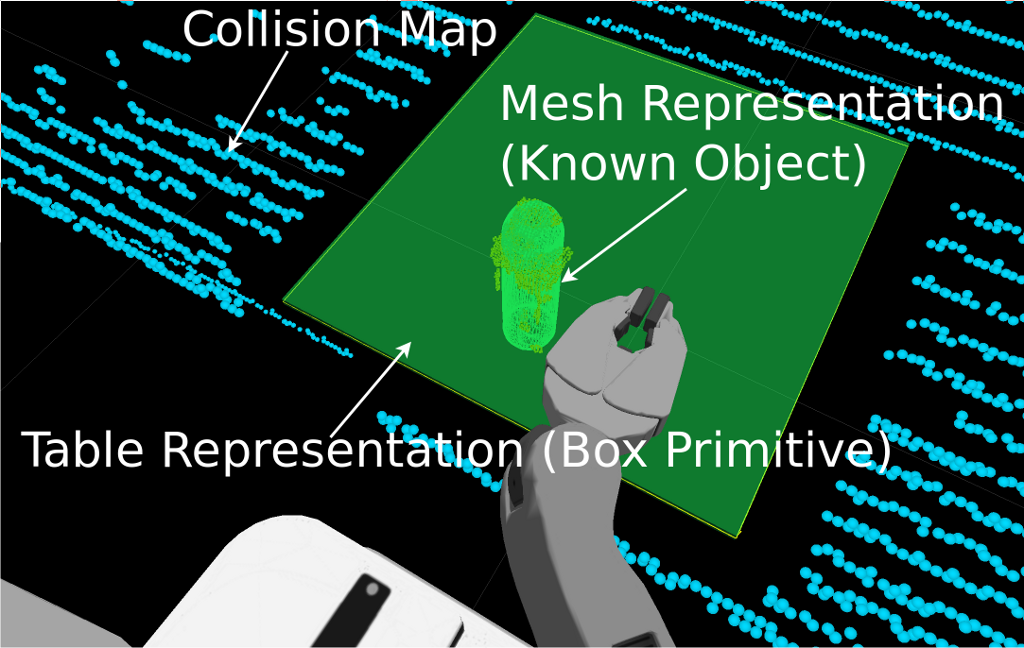
\includegraphics[width=0.45\linewidth]{figs/7/labeled_small.png}
  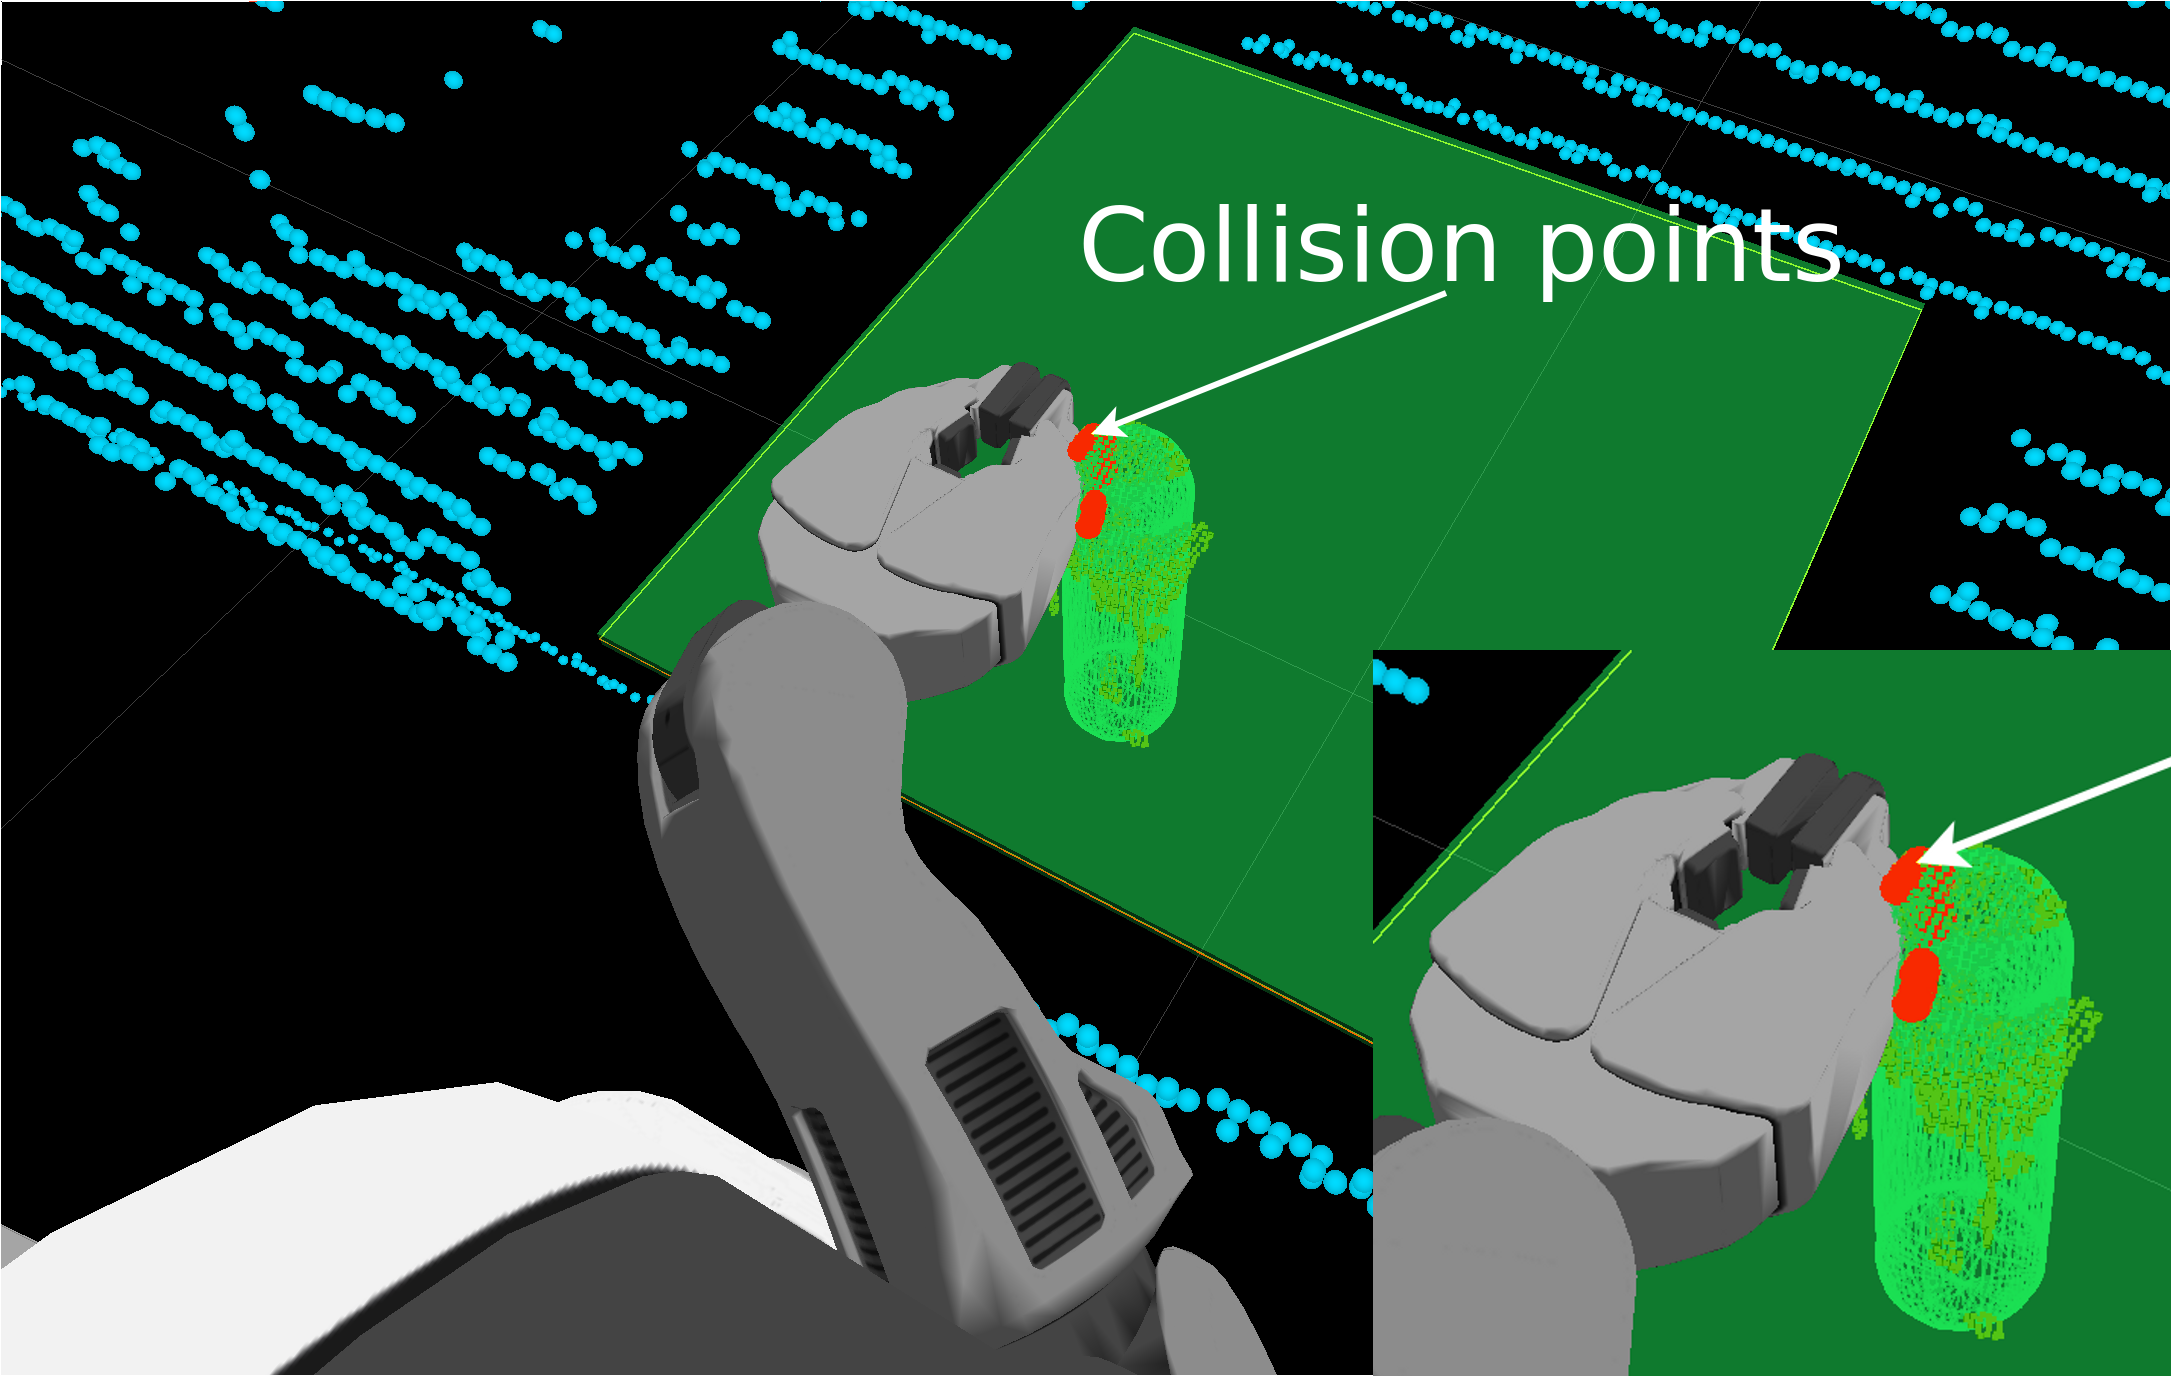
\includegraphics[width=0.45\linewidth]{figs/7/labeled_in_collision_pip.png}
  \caption[A visual representation of the collision information generated by the sensors on the PR2 robot]{\label{fig:7:pr2} A visual representation of the collision information generated by sensors on the PR2 robot. (Left) The environment includes the points in a collision map (in light blue), mesh representations for known objects detected through visual sensing (the green cylindrical object on table), and an exact geometric representation of the table surface (the green flat surface). A detailed mesh model for the robot is also seen in the picture. (Right) A representation of the collision points (shown by red spheres) between the gripper and the object on the table.
We use our probabilistic algorithm for robust collision checking with noisy point clouds at interactive rates.}
\end{figure}

The rest of this chapter is organized as follows. We survey related work in Section~\ref{sec:7:related}.  We introduce our notation and give an overview of the approach in
Section~\ref{sec:7:overview}.
Section~\ref{sec:7:algorithm} shows how probabilistic collision detection computation is reduced to robust classification and Section~\ref{sec:7:bvh} describes the use of bounding volume hierarchies to accelerate the
computation.
We evaluate the performance of our algorithm on different benchmarks in Section~\ref{sec:7:results}.

\section{Related Work}
\label{sec:7:related}
The field of probabilistic robotics provides a mathematical framework for handling the uncertainty that exists
in the physical world~\cite{PR:2005}.  It deals with representing uncertainty explicitly using the calculus of probability distribution
and obtaining robust control choices relative to the uncertainty in the robot system. Probabilistic robotics can handle perception uncertainty (or environment uncertainty) due to sensor and action errors. However, previous approaches tend to use simple methods to model environment uncertainty, such as feature-based methods or occupancy grid based methods. These models can only provide a rough description of the environment, while many robot actions (e.g., grasping) require more detailed information for robust computation.

\subsection{Uncertainty of Point Cloud Data}
\label{sec:7:related:data}
Raw point cloud data obtained from sensors can have a high degree of uncertainty, which results mainly from
discretization error and noise. As a result, it is difficult to obtain robust estimation of high-order features such as surface normals. This causes difficulty for many applications that require precise estimates of normal vectors at the boundary, such as grasping.

Many approaches consider uncertainty of point clouds implicitly. For example, \cite{Steinke:2005,Bernhard:2005nips} encode surface uncertainty as a parameter tolerance for learning algorithms when they apply geometric operations (e.g., reconstruction) on the point clouds. However, without an explicit model of uncertainty, we can only consider a single uncertainty formulation for the overall surface, so we may not be able to model varying uncertainty at different parts of the surface for local control.

There is recent work on explicitly modeling the uncertainty of point cloud data for different applications. \cite{Bae:2009} present a closed-form expression for the positional uncertainty of point clouds. \cite{Pauly:2004} propose two methods, confidence map and likelihood map, to analyze shape uncertainty in
point clouds for re-sampling and reconstruction applications. \cite{Jenke:2006} describe a Bayesian model for incorporating point cloud uncertainty
in surface reconstruction.

\subsection{Collision Detection}
In order to handle the interaction between point cloud data, we need efficient and accurate collision detection algorithms between point cloud data; these algorithms should take into account the uncertainty of point cloud data in a formal manner.
However, prior collision detection methods mainly focus on performing efficient and accurate contact computations between objects represented by triangulated primitives~\cite{LM03}.

In terms of collision checking with point clouds, there are several simple methods. For example,
we can first reconstruct triangle meshes from point clouds and then perform exact collision checking between the reconstructed surfaces.
However, this approach suffers from inefficiency ($>10$ s for 10K points) and robustness issues that arise from using reconstruction algorithms (e.g., reconstruction quality, sensitiveness to parameter and noise, etc). We can also simply expand every point as a sphere with suitable radius and approximate the object as a union of spheres~\cite{Hubbard:1996} for collision checking. The main difficulty with this approach is automatically choosing different sphere radii for different points. Other direct collision checking methods for point cloud data are based on using bounding volume hierarchies~\cite{Jan:2004,Sternemann:2007} and reconstructing implicit functions at the leaf nodes, which are also prone to robustness issues. Minkowski sums of point clouds have also been used for collision queries~\cite{Lien:2007}. \cite{Ioan:2010} describe a collision map data structure, which uses axis aligned cubes to model the point cloud and to perform collisions with a robot.
Some applications, including virtual reality and haptics, need real-time collision checking, and use probabilistic criteria based on minimum distance computation between the point sets~\cite{Lee:haptics:2007}. However, these methods do not take into account the inherent shape uncertainty of point cloud data that arises from discretization or sampling~\cite{Pauly:2004}.

There has been relatively little work in terms of handling uncertainty in collision detection. A special type of collision uncertainty is discussed in~\cite{Govindaraju:2006:VRST}, which projects objects onto different image planes to perform collision culling using GPU-based computation. \cite{Guibas:wafr2009} propose a method to compute the collision probability between 2D objects composed of line segments in a 2D environment with uncertainty. In order to estimate collision uncertainty, this method models the endpoints of a line segment as probability distributions with a rectangular support region. \cite{Missiuro:2006} also try to model uncertainty in probabilistic roadmaps by using the collision probability of a configuration to bias the sampling process for roadmap computation.


\section{Overview}
\label{sec:7:overview}
In this section we introduce the notation used in the rest of the chapter and give an overview of our approach.

The main \emph{pipeline} of our system
consists of three steps: 1) Obtain raw data from sensors and filter the point clouds to remove points on the robot and reduce the shadow effect~\cite{Ioan:2010}; 2) Compute the separating surface between two point clouds by estimating the noise from sensor parameters (Sections~\ref{sec:7:algorithm:1}-\ref{sec:7:algorithm:3}); and 3) Estimate the collision probability for each point and the overall collision probability between two point clouds (Section~\ref{sec:7:algorithm:4}). Moreover, we use bounding volume hierarchies to accelerate the computation and recompute the hierarchies for dynamic environments (Section~\ref{sec:7:bvh}).

The inputs to our collision detection algorithm are the point clouds. In some cases, we need to perform
the collision query between two different point clouds or between a point cloud and a polygonal object (e.g., when the mesh representation of a robot hand or gripper is available). We first present our
approach for two different point clouds, and later show how it can be applied to a point cloud and a polygonal object.

Let the two point clouds be denoted as $C_1$ and $C_2$.
We assume that each point cloud $C$ is obtained from sensors and is a partial
and noisy representation of the underlying exact surface $S$. There are two kinds of errors introduced in the generation of point clouds: \emph{discretization errors}
and \emph{position errors}, or \emph{noise uncertainty}. Intuitively, discretization error refers to how these point samples are distributed on the boundary of the surface, and the position error measures the imprecision in the coordinates of each point. Formally, we assume $C$ is generated from $S$ according to the following process: first a series of $n$ sample
points $\mathbf x_i'$ is generated according to some sampling process and we use the symbol $p(\mathbf x_i'|S)$ to represent the distribution of coordinates for a random point $\mathbf x_i'$; this models the discretization error. Next, $\mathbf x_i$ is generated from $\mathbf x_i'$
according to some noise distribution $p(\mathbf x_i|\mathbf x_i'; \Sigma_i)$; this models the position error. Generally $p(\mathbf x_i' |S)$ is not given, but we can estimate it based on the observed point-cloud data, with some assumptions about surface smoothness and sampling density. The symbol $\Sigma_i$ is used to model a point cloud's uncertainty due to noise, and is typically computed based on sensor characteristics. For example, $\Sigma_i$ may measure the level of noise that is a combination of sensing noise, motion uncertainty, and deformation error. Then the overall uncertainty of a point $\mathbf x_i$ can be modeled as
\begin{equation}
\label{eq:7:point-model}
\mathbf x_i|S \sim p(\mathbf x_i|S) = \int p(\mathbf x_i'|S)p(\mathbf x_i|\mathbf x_i'; \Sigma_i) \ d\mathbf x_i'.
\end{equation}
In this formulation, there exists an implicit assumption that the sensor is able to capture the features of the underlying surface. For example, more sample points $\mathbf x_i'$ must be generated near the sharp features, so that we can reconstruct the necessary features of the original model.

The output of the collision detection algorithm is a probability $\mathbb{P}_{C_1, C_2}$ that estimates whether two point clouds $C_1$ and $C_2$ are in-collision.

\subsection{Separating Surface}
\label{sec:7:overview:2}
Given a point cloud, we can potentially reconstruct a triangulated surface representation using Bayesian optimization. That is, the underlying surface should be the one with the maximum probability:
\begin{equation}
\hat{S} = \argmax_S p(S|\{\mathbf x_i\}_{i=1}^n) = \argmax_S p(S) \prod_i p(\mathbf x_i | S).
\end{equation}
Next, we can perform collision checking based on reconstructed models. However, reconstructions are only estimations, so computing collisions based on reconstructions can be rather inaccurate.
Our formulation is based on the theory of convex sets: two convex sets are non-intersecting if there exists an oriented \emph{separating plane} $P$ so that one set is completely in the positive (open) halfspace $P^+$ and the other is completely in the negative (open) halfspace $P^-$~\cite{Mount:2004}. For non-convex sets, we extend the concept of the separating plane to the \emph{separating surface}: two sets are non-intersecting (or \emph{separable}) if and only if there exists a separating surface $P$ between them. Previous work in collision detection~\cite{Mount:2004, Ponamgi:1995} is limited to the special case when $P$ is composed of multiple planes.

We extend the idea of separating surfaces to handle point clouds. Given two point clouds $C_1 = \{\mathbf x_i^1\}_{i=1}^{n_1}$ and $C_2 = \{\mathbf x_i^2\}_{i=1}^{n_2}$
with $n_1$ and $n_2$ elements, respectively, a separating surface $P$ is a surface that can separate the two sets completely with $C_1$ in $P^+$ and $C_2$ in $P^-$.
In this case, $P^+$ and $P^-$ represent a partition of the space $\Rcubic$ into two parts. Notice that here $P$ should not be an
arbitrary surface: i.e., it should not be a very complex function in terms of acting as a valid separating surface. Otherwise, even if $P$ can completely separate the point clouds, it may not be able to separate the underlying surfaces. Such a problem is called \emph{overfitting} in machine learning literature, which describes when the statistical model is biased too much towards the observed data and thus may not be able to predict the underlying model correctly. In order to avoid overfitting, we assume \emph{regularity conditions} for $P$, which intuitively impose suitable smoothness constraints on the separating surface. In our algorithm, we represent $P$ as a parameterized implicit surface $\{\mathbf x: f(\mathbf x; \theta) = 0\}$ with $\theta$ as its parameters. In this case, the regularity condition can limit the value of $f'(\mathbf x; \theta)$. Moreover, $P^+$ and $P^-$ can be represented as $\{\mathbf x: f(\mathbf x; \theta) > 0\}$ and $\{\mathbf x: f(\mathbf x; \theta) < 0\}$, respectively. As a result, the collision detection problem is reduced to finding the separating surface, i.e., deciding the parameter set $\theta$, that can separate $C_1$ and $C_2$.

There is one major difference between point clouds and convex/non-convex sets. In particular, for point cloud data, the existence of a separating surface is \emph{not} a necessary or sufficient condition for non-intersection between the two sets. If two point clouds are noise-free and separable, their underlying surfaces may still be in-collision, as shown in Figure~\ref{fig:7:separating-point}(a)-(b). This is due to the discretization error from point-cloud sampling. This issue becomes more complicated when point clouds have position errors, as shown in Figure~\ref{fig:7:separating-point}(c)-(d).
This property of point cloud sets makes it difficult to perform exact collision checking, but is suitable for statistical learning approaches like SVM~\cite{Bi:2005}. As a result, the probabilistic collision detection problem can be reduced to computing the optimal separating surface that minimizes the \emph{separating error}
for underlying surfaces: i.e., find $\theta$ that minimizes
\begin{equation}
\label{eq:7:error}
\int_{\mathbf x \in S_1} \mathbf{1}_{\{\mathbf x \in P(\theta)^-\}} \ d\mathbf x + \int_{\mathbf x \in S_2} \mathbf{1}_{\{\mathbf x \in P(\theta)^+\}} \ d\mathbf x,
\end{equation}
where $S_1$ and $S_2$ are the underlying surfaces for point clouds $C_1$ and $C_2$, respectively.


\begin{figure}[!htb]
  \centering
  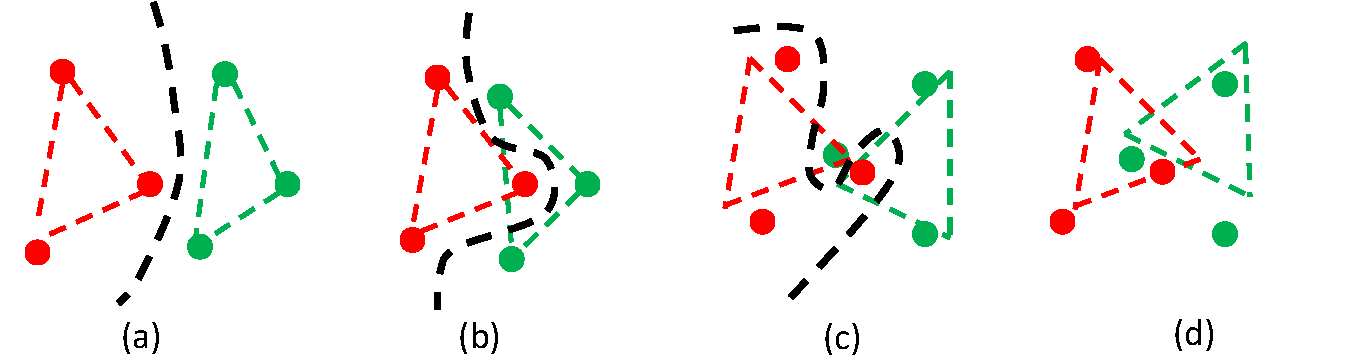
\includegraphics[width=0.9\linewidth]{figs/7/separating-point.pdf}
  \caption[Separating surface for point cloud sets]{\label{fig:7:separating-point} Separating surface for point cloud sets. Point clouds in (a) and (b) are noise-free and are separable. However, due to discretization uncertainty, the underlying surfaces can be either
  collision-free (a) or in-collision (b). Point clouds in (c) and (d) have some noise and may not be separable, and the underlying surfaces can be either collision-free (c) or in-collision (d). Notice that we require suitable regularity or smoothness on the separating surface to avoid overfitting. For example, the separating surface provided in (c) has too large of a curvature and therefore is not valid. Thus, collision results based on reconstructed meshes may not be reliable due to discretization error, as in examples (a) and (b), or position noise, as in examples (c) and (d), or unsuitable parameters.}
\end{figure}


\subsection{Probabilistic Model for Point Cloud Collision}
We now present the probabilistic model for using point cloud collision checking to compute the optimal separating surface. We rewrite $\mathbf x_i^l$ with $l\in \{1,2\}$ as $(\mathbf x_i, c_i)$, where $\mathbf x_i = \mathbf x_i^l$ and $c_i = (-1)^{l+1} \in \{-1, 1\}$ denotes which object the point $\mathbf x_i$ belongs to.
As a result, we have $n_1 + n_2$ elements in $\{(\mathbf x_i, c_i)\}$. As discussed in Section~\ref{sec:7:overview:2}, collision checking between two point sets reduces
to finding an optimal separating surface $P$. In machine learning terminology, this corresponds to finding an optimal classifier that can minimize the expected risk on the classification problem whose data is drawn
from $\{ \mathbf x: \mathbf x \in S_1 \bigcup S_2\}$ and its {\em training set} is $\{(\mathbf x_i, c_i)\}$. As a result, the collision detection problem is reduced to a
machine learning problem. However, unlike typical machine learning algorithms only dealing with cases in which $(\mathbf x_i, c_i)$ are specified exactly, we also need to take into account the noise in $\mathbf x_i$. Our solution is based on the maximum-likelihood (ML) scheme, which chooses the optimal surface to maximize the probability on the observed inputs $\{(\mathbf x_i, c_i)\}$.

Similar to Equation~\ref{eq:7:point-model}, the joint probability for $(\mathbf x_i, c_i)$ can be expressed as
\begin{equation}
p(\mathbf x_i, c_i) = \int p(\mathbf x_i', c_i; \theta) p(\mathbf x_i|\mathbf x_i'; \Sigma_i) \ d\mathbf x_i'.
\end{equation}
Here $\theta$ is the parameter set used to represent the separating surface $P$. For example, $P$ is $\{\mathbf x: \mathbf w^T \mathbf x + b = 0\}$ if $P$ is a plane and $\theta = \{\mathbf w, b\}$. Or, $P$ is $\{\mathbf x: \mathbf w^T \Phi(\mathbf x) + b = 0\}$ if $P$ is a hyper-plane in some high-dimensional inner product space $\mathcal H$ and $\Phi$ is the mapping $\Phi: \Rcubic \mapsto \mathcal H$. The unknown surface parameter $\theta$ can be estimated from the point cloud data using ML:
\begin{equation}
\begin{aligned}
\label{eq:7:point-collision}
\theta^*
%= \argmax_{\theta}\sum_i \ln p(\mathbf x_i, c_i) \\
&= \argmax_{\theta} \sum_i \ln \int p(\mathbf x_i', c_i; \theta) p(\mathbf x_i|\mathbf x_i'; \Sigma_i) \ d\mathbf x_i'
\end{aligned}
\end{equation}
In practice, the integration over the unknown underlying surface sample $\mathbf x_i'$ makes it hard to compute the surface parameter. As a result,
we consider an alternative form that is computationally more efficient. Specifically, we use an approximation to Equation~\ref{eq:7:point-collision}
based on a widely-used heuristic for mixture estimation: we simply regard $\mathbf x_i'$ as a parameter of the model instead of a random variable. Then Equation~\ref{eq:7:point-collision} reduces to:
\begin{equation}
\label{eq:7:point-collision:2}
\theta^* = \argmax_{\theta} \sum_i \ln \sup_{\mathbf x_i'} p(\mathbf x_i', c_i; \theta) p(\mathbf x_i|\mathbf x_i'; \Sigma_i).
\end{equation}
We present an algorithm to solve Equation~\ref{eq:7:point-collision:2} in the following section.


\section{Probabilistic Collision Checking between Point Clouds}
\label{sec:7:algorithm}
In this section, we present our probabilistic algorithm for collision checking between point clouds using two-class classification. This reduces to computing the optimal separating surface that minimizes the function in Equation~\ref{eq:7:point-collision:2}.


\subsection{Basic Formulation}
\label{sec:7:algorithm:1}
For convenience, we first assume that the separating surface is a plane, i.e., $P = \{\mathbf x: \mathbf w^T \mathbf x + b = 0\}$. We also assume that the uncertainty due to noise can be described by a Gaussian distribution. We will relax these assumptions later on.
Based on these two assumptions, we have
\begin{equation}
p(\mathbf x_i', c_i; \theta) \sim p(\mathbf x_i') \exp(-\frac{(\mathbf w^T \mathbf x_i' + b - c_i)^2}{\sigma^2}) 
\end{equation}
and
\begin{equation}
p(\mathbf x_i | \mathbf x_i'; \Sigma_i) \sim \exp(-(\mathbf x_i - \mathbf x_i')^T \Sigma_i^{-1} (\mathbf x_i - \mathbf x_i')),
\end{equation}
where $\sigma$ and $\Sigma_i$ are the covariance parameters of a Gaussian distribution.

As we will show in Section~\ref{sec:7:results}, the discretization uncertainty at $\mathbf x_i'$ can also be estimated as a Gaussian distribution with the observation $\mathbf x_i$ as the mean. That is, $p(\mathbf x_i') \sim \exp(-(\mathbf x_i' - \mathbf x_i)^T \Psi_i^{-1} (\mathbf x_i' - \mathbf x_i))$, where $\Psi_i$ is the covariance parameter for discretization uncertainty. Here we assume that the observed data $\mathbf x_i$ is fixed and the true value $\mathbf x_i'$ is subject to random errors. This is equivalent to the so-called \emph{Berkson's model} in statistics literature~\cite{Berkson:1950}.
Then Equation~\ref{eq:7:point-collision:2} becomes
\begin{equation}
\label{eq:7:point-collision:3}
\theta^* = \argmax_{\theta} \sum_i \inf_{\mathbf x_i'} \Big[\frac{(\mathbf w^T \mathbf x_i' + b - c_i)^2}{\sigma^2} + (\mathbf x_i - \mathbf x_i')^T \widetilde{\Sigma}_i^{-1} (\mathbf x_i - \mathbf x_i')\Big],
\end{equation}
where $\theta = \{\mathbf w, b\}$ and $\widetilde{\Sigma}_i^{-1} = \Sigma_i^{-1} + \Psi_i^{-1}$.

Moreover, notice that if $(\mathbf x_i - \mathbf x_i')^T \widetilde{\Sigma}_i^{-1} (\mathbf x_i - \mathbf x_i')$ is large, then the $p(\mathbf x_i', c_i; \theta)$ term
will have a small value and can be ignored in the integration for $p(\mathbf x_i, c_i)$. As a result, we can constrain $\mathbf x_i'$ to lie within the
ellipsoid $\mathcal{E}_i = \{\mathbf x_i': (\mathbf x_i - \mathbf x_i')^T \widetilde{\Sigma}_i^{-1} (\mathbf x_i - \mathbf x_i') \leq r_i^2\}$ and this will not influence
the final result considerably. Also, considering the regularity of separating surfaces, Equation~\ref{eq:7:point-collision:3} can be approximated by an optimization
formulation that is similar to that used for the support vector machine (SVM):
\begin{equation}
\label{eq:7:point-collision:4}
\begin{aligned}
	& \underset{\mathbf w, b, \xi_i}{\text{minimize}}
	& & \frac{1}{2}\|\mathbf w\|^2 + \lambda \sum_{i=1}^n \xi_i \\
	& \text{subject to}
	& & c_i(\mathbf w^T \mathbf x_i' + b) \geq 1 - \xi_i, & \forall \mathbf x_i' \in \mathcal{E}_i, \forall 1 \leq i \leq n; \\
    & & & \xi_i \geq 0, & \forall 1 \leq i \leq n,
	\end{aligned}
	\end{equation}
The above formulation minimizes the upper bound on the classification error, which is equivalent to the separating error in Equation~\ref{eq:7:error}. Errors occur when $\xi_i \geq 1$, as $\mathbf x_i'$ lies on the wrong side of $P$. The quantity $\lambda$ is the penalty for any data point $\mathbf x_i'$ that either lies within the margin on the correct side of $P$ ($0 < \xi_i \leq 1$) or on the wrong side of $P$ ($\xi_i > 1)$. $\|\mathbf w\|$ is the regularization term which controls the smoothness of the separating surface.

It is easy to verify that $c_i(\mathbf w^T \mathbf x_i' + b)$ reaches its minimum at point $\mathbf x_i - r_i (\mathbf w^T \widetilde{\Sigma}_i \mathbf w)^{1/2}\widetilde{\Sigma}_i \mathbf w$ and the minimum value is $c_i(\mathbf w^T \mathbf x_i + b) - r_i (\mathbf w^T \widetilde{\Sigma}_i \mathbf w)^{1/2}$.   As a result,
Equation~\ref{eq:7:point-collision:4} can be further written as:
\begin{equation}
\label{eq:7:point-collision:5}
\begin{aligned}
	& \underset{\mathbf w, b, \xi_i}{\text{minimize}}
	& & \frac{1}{2}\|\mathbf w\|^2 + \lambda \sum_{i=1}^n \xi_i \\
	& \text{subject to}
	& & c_i(\mathbf w^T \mathbf x_i + b) \geq 1 - \xi_i + r_i \|\widetilde{\Sigma}_i^{1/2} \mathbf w \|, & \forall 1 \leq i \leq n; \\
    & & & \xi_i \geq 0, & \forall 1 \leq i \leq n.
	\end{aligned}
	\end{equation}
Such optimization problems have been studied in the literature~\cite{Shivaswamy:2006:SOC} and can be solved using second order cone programming (SOCP)
methods. Once $\mathbf w$ and $b$ are computed, we can compute $\xi_i = \max(0, 1 - c_i(\mathbf w^T \mathbf x_i + b) + r_i \|\widetilde{\Sigma}_i^{1/2}\mathbf w\|)$.


\subsection{Non-Gaussian Uncertainty}
\label{sec:7:algorithm:2}
The uncertainty of real-world sensors may not be accurately modeled using a Gaussian distribution. Our approach can also handle non-Gaussian uncertainty.

\cite{Shivaswamy:2006:SOC} point out that the ellipsoid radius $r_i$ is related to the confidence of the classification result when the training data contains noise. Briefly, if we desire the underlying surface point $\mathbf x_i'$ with a Gaussian distribution to lie on the correct side of the separating surface with a probability greater than $\kappa_i$; i.e.,
\begin{equation}
\mathbb{P}_{\mathbf x_i'\sim \mathcal{N}(\mathbf x_i, \widetilde{\Sigma}_i)}\Big((c_i(\mathbf w^T \mathbf x_i' + b) \geq 1 - \xi_i\Big) \geq \kappa_i,
\end{equation}
then $r_i = \erf^{-1}(\kappa_i)$, where $\erf(u) = \frac{1}{\sqrt{2\pi}}\int_{-\infty}^{u}\exp(-\frac{s^2}{2})ds$.
Applying the multivariate Chebyshev inequality, this relationship between $\kappa_i$ and $r_i$ can be further extended to the case when $\mathbf x_i'$ follows non-Gaussian distribution. That is, if $\mathbf x_i' \sim (\mathbf x_i, \widetilde{\Sigma}_i)$ represents a family of distributions with a common mean and covariance given by $\mathbf x_i$ and $\widetilde{\Sigma}_i$, and we want $\mathbf x_i'$ to lie on the correct side of the separating surface with a probability greater than $\kappa_i$; i.e.,
\begin{equation}
\sup_{\mathbf x_i' \sim (\mathbf x_i, \widetilde{\Sigma}_i)} \mathbb{P}_{\mathbf x_i'}\Big((c_i(\mathbf w^T \mathbf x_i' + b) \geq 1 - \xi_i\Big) \geq \kappa_i,
\end{equation}
then $r_i = \sqrt{\frac{\kappa_i}{1-\kappa_i}}$. This formulation implies that we can perform collision detection using Equation~\ref{eq:7:point-collision:5}
even when the uncertainty is non-Gaussian.


\subsection{Non-linear Separating Surface}
\label{sec:7:algorithm:3}

Using a linear separating surface is mainly limited to the case when all the underlying surfaces are convex. If any one of them is non-convex, a separating plane may not exist even when
the surfaces are collision-free. Therefore, we need to extend our algorithm to non-linear $P$. Similar to typical SVM algorithms~\cite{Vapnik:1995:NSL}, we can remove the linear separating surface assumption by applying a {\em kernel trick} on the
dual form of Equation~\ref{eq:7:point-collision:5}. Briefly, the kernel trick is a method that transforms the Euclidean space $\mathcal{R}^n$ into an
inner space $\mathcal{H}$ using the mapping $\Phi$, replacing the inner product $\langle \mathbf y, \mathbf z \rangle_{\mathcal{R}^n}$ by the new inner product $K(\mathbf y, \mathbf z) = \langle \Phi(\mathbf y), \Phi(\mathbf z) \rangle_{\mathcal{H}}$ in space $\mathcal{H}$.
Here $K(\cdot, \cdot)$ is called the {\em kernel function}. Usually a hyper-plane in $\mathcal{H}$ will correspond to a non-linear surface in $\mathcal{R}^n$, which is a popular way to construct non-linear classifiers in machine learning~\cite{Hofmann:2008}. A couple of widely-used kernel functions include the linear ($K(\mathbf y, \mathbf z) = \mathbf y^T \mathbf z$) and Gaussian ($K(\mathbf y, \mathbf z) = \exp(-\gamma \|\mathbf y - \mathbf z\|^2)$) kernels.

Based on the kernel trick, the non-linear separating surface can be formulated as $P = \{\mathbf x: \mathbf w^T \Phi(\mathbf x) + b = 0\}$. To compute $P$,
we first transform Equation~\ref{eq:7:point-collision:5} into its dual form. Next, based on the Taylor-expansion technique~\cite{Bi:2005}, we replace $\mathbf y^T \mathbf z$ by kernel function $K(\mathbf y, \mathbf z)$ and
replace $\mathbf y$ by the kernel gradient $\frac{\partial K(\mathbf y, \mathbf z)}{\partial \mathbf z}$ and finally obtain the optimization formulation in the non-linear case as
\begin{equation}
\label{eq:7:point-collision:6}
\begin{aligned}
	& \underset{\mathbf \alpha_i, \mathbf v_i}{\text{maximize}}
	& & \sum_{i=1}^n \alpha_i - \frac{1}{2}\Big( \sum_{i=1}^n \sum_{j=1}^n \alpha_i \alpha_j c_i c_j K(\mathbf x_i, \mathbf x_j) + \sum_{i=1}^n \sum_{j=1}^n \alpha_i c_i \big( \widetilde{\Sigma}_j^{1/2} \frac{\partial K(\mathbf x_i, \mathbf x_j)}{\partial \mathbf x_j}\big)^T \mathbf v_j  \\
    & & &  + \sum_{i=1}^n \sum_{j=1}^n \alpha_j c_j \big( \widetilde{\Sigma}_i^{1/2} \frac{\partial K(\mathbf x_i, \mathbf x_j)}{\partial \mathbf x_i}\big)^T \mathbf v_i + \sum_{i=1}^n \sum_{j=1}^n \mathbf v_i^T \big( \widetilde{\Sigma}_i^{1/2} \frac{\partial^2 K(\mathbf x_i, \mathbf x_j)}{\partial \mathbf x_i \partial \mathbf x_j} \widetilde{\Sigma}_j^{T/2}\big) \mathbf v_j \Big) \\
	& \text{subject to}
	& & \|\mathbf v_i\| \leq r_i \alpha_i, \ 0 \leq \alpha_i \leq C, \ \forall 1 \leq i \leq n; \ \text{and} \ \sum_{i=1}^n \alpha_i c_i = 0;  \\
	\end{aligned}
	\end{equation}
where $C$ is a regularity term similar to $\lambda$ in Equation~\ref{eq:7:point-collision:5}. Once $\alpha_i$ and $\mathbf v_i$ are computed, we can compute
the formulation for the separating surface $P$ as
\begin{equation}
f(\mathbf x) = b + \sum_{j=1}^n \alpha_j c_j K(\mathbf x_j, \mathbf x) + \sum_{j=1}^n \mathbf v_j^T \widetilde{\Sigma}_j^{1/2} \frac{\partial K(\mathbf x_j, \mathbf x)}{\partial \mathbf x_j}
\end{equation}
and $\xi_i = \max(0, \xi_i')$, where
\begin{equation}
\label{eq:7:error:kernel}
\xi_i' = 1 - c_i f(\mathbf x_i) + r_i \|\widetilde{\Sigma}_i^{1/2} f'(\mathbf x_i)\|.
\end{equation}
Notice that the surface parameter $b$ does not appear in the dual form, but it can be computed based on Karush--Kuhn--Tucker conditions~\cite{CC01a}.
We first choose $i$ so that $0 < \alpha_i < C, \|\mathbf v_i \| < r_i \alpha_i$, and then set $\xi_i' = 0$ in Equation~\ref{eq:7:error:kernel} to obtain $b$.
Moreover, notice that all the results for non-linear separating surfaces are consistent with those for linear separating surfaces, which use the
linear kernel $K(\mathbf y, \mathbf z) = \mathbf y^T \mathbf z$.


\subsection{Probabilistic Collision Decision}
\label{sec:7:algorithm:4}

Based on the computed separating surface, we present a simple scheme to perform probabilistic collision detection between the point clouds.
First, we compute the collision probability for each point, i.e., the probability that $\mathbf x_i'$ lies on the wrong side of separating surface:
\begin{equation}
\label{eq:7:perpointcolprob}
\mathbb{P}_{\mathbf x_i' \sim \mathcal{N}(\mathbf x_i, \widetilde{\Sigma}_i)} (c_i f(\mathbf x_i') \leq 0) =
\erf(-c_i f(\mathbf x_i) / \|\widetilde{\Sigma}_i^{1/2} f'(\mathbf x_i)\|).
\end{equation}
We denote this per-point probability as $\mathbb{P}(\mathbf x_i)$.
Next, we need to use an appropriate metric to measure the collision probability between two point clouds.
For two exact models, collision occurs if \emph{any} subsets of them are in-collision. Therefore, for point clouds $C_1$ and $C_2$, it seems reasonable to define the collision probability between them as $1 - \prod_{\mathbf x \in \{C_1 \bigcup C_2\}} [1 - \mathbb{P}(\mathbf x)]$. However, this metric has some problems: when the number of points increases, its value will go to zero instead of converging to the real collision probability. The reason for this is that this metric does not consider the dependency between collision states of nearby points.
In contrast, our approach for computing collision probability only involves far-away points with large per-point collision probabilities.
First, we compute the maximum per-point collision probability $\max_{\mathbf x} \mathbb{P}(\mathbf x)$. Next, we find all the points whose per-point collision probabilities are near the maximum value, e.g., more than $0.8 \max_{\mathbf x} \mathbb{P}(\mathbf x)$. For points that are close to each other, we only use one of them in the whole body collision probability computation. The first rule filters out points whose collision probabilities are not large enough to improve the stability of collision results, while the second rule filters out points that are closely correlated. Finally, we compute the collision probability between point clouds based on the left $m \ll n$ points $\{\tilde{\mathbf x}_i\}$: $\mathbb{P}_{C_1, C_2} = 1 - \prod_{i=1}^m [1 - \mathbb{P}(\tilde{\mathbf x}_i)]$. We can also use a simpler version of this metric, which only considers the point with the maximum collision probability: $\mathbb{P}_{C_1, C_2} = \max_{\mathbf x \in C_1 \bigcup C_2} \mathbb{P}(\mathbf x)$. For collision between exact models, the two metrics are equivalent, as $\mathbb{P}(\tilde{\mathbf x}_i) = \max_{\mathbf x} \mathbb{P}(\mathbf x) = 1$,
for all $i$. The simpler metric can not distinguish the collision states when point clouds have one or more
far-away points with large per-point collision probability, but it is more efficient for distinguishing between collision-free and in-collision cases.


\subsection{Handling Polygonal Objects}
In many cases, the exact mesh representation of one of the objects is known (e.g., the model of the robot operating in the environment).
We assume that the object is represented using a triangle mesh and we extend our point-cloud algorithm to handle such models.
It turns out that we only need to represent a triangle by four noise-free points: three vertices and the centroid point.
The regularity of a separating surface guarantees that if these four points are separated from the other point cloud (say $C_1$)
then the entire triangle lies on one side of the separating surface.
Thus, we can use the framework above to compute the collision probability; the only difference is that we
set $r_i = 0$ and use a larger value for $\lambda$ or $C$ in Equation~\ref{eq:7:point-collision:6} for the points from the triangles, to bias
the optimization solver to minimize the error for the points that lie on the triangles. The collision probability for a noisy point
can still be computed by Equation~\ref{eq:7:perpointcolprob}, while the collision probability for any exact point is equal to
$1$ if it lies on the wrong side of the separating surface.


\section{Acceleration using Bounding Volume Hierarchies}
\label{sec:7:bvh}


We have reduced the problem of collision detection between two point clouds to a two-class classification problem and can solve it with SVM. However, performing
collision detection by directly using Equation~\ref{eq:7:point-collision:6} introduces some challenges. First, the time complexity of SVM can be $\mathcal O(n^3)$,
where $n = n_1 + n_2$ is the total number of points in the two point clouds. As a result, the underlying algorithm can be slow for dense point clouds.
Second, the two point clouds corresponding to different objects may have different numbers of points, which can result in unbalanced training data.
Moreover, if the two point clouds under consideration correspond to objects with different sizes (e.g., a large room and a small robot), it will cause the optimization algorithm to have a lower separating error for the larger object and higher error for the smaller object.

We use bounding volume hierarchies (BVH) to overcome these problems. These hierarchies quickly identify objects or parts of an object that can be easily culled away, and therefore perform exact collision queries on relatively
few primitives.
In our algorithm, each leaf node of our BVH contains a subset of the point clouds. The BVH is computed in a top-down manner, and we terminate the BV split recursion according to
the covariance of points and the number of points within the given BV. For each BV, we compute the covariance matrix $\mathbf C = \frac{1}{m} \sum_{i=1}^{m} (\mathbf x_i - \overline{\mathbf x})(\mathbf x_i - \overline{\mathbf x})^T$, where $\{\mathbf x_i\}_{i=1}^m$ are the points in the BV and $\overline{\mathbf x}$ is their mean.
Next, we compute $\mathbf C$'s three eigenvalues $\sigma_1, \sigma_2, \sigma_3$, assuming $\sigma_1 \leq \sigma_2 \leq \sigma_3$. We define $\sigma_n = \frac{\sigma_1}{\sigma_1 + \sigma_2 + \sigma_3}$ as the BV's variation, where $0 \leq \sigma_n \leq 1/3$. $\sigma_n = 1/3$ means points in the BV are completely isotropically distributed, while $\sigma_n = 0$ means all these points lie in a plane. We continue splitting the given BV along its longest axis (i.e., the eigenvector of $\mathbf C$ corresponding to $\sigma_3$) if the number of points it contains is larger than $n_{max}$ or the corresponding $\sigma_n$ is above $\sigma_{max}$, where $n_{max}$ and $\sigma_{max}$
are two thresholds.

In prior BVH-based algorithms for triangulated models, the children nodes split from the same parent node will typically have no common triangles.
However, for point clouds, the BVH constructed in this manner will result in false negatives (i.e., missed collisions). As shown in Figure~\ref{fig:7:bvh_overlap}(a), the BVs
of two objects can be collision-free even when the underlying surfaces are non-separable, and the algorithm will return incorrect an collision-free result
without checking for collisions between any leaf nodes. To overcome this problem,  we require BVs split from the same parent to contain $\epsilon$-overlap with
each other. We usually set $\epsilon$ to be $1\%- 5\%$. Such an overlap will result in some redundancy in terms of point storage: for one object with $n$ points, its
BVH will store about $(1+\epsilon \ln \frac{n}{n_{max}} ) n$ points, where $n_{max} > 1$ is the threshold used in BV splitting.


In the case of point clouds, a BVH may not fully enclose the point primitives that lie within it.
There is a small probability that the underlying surface may not be completely enclosed. Thus, even if two nodes are non-intersecting, we still need to check the collision between the point clouds within them with a small probability. We call this probability the \emph{leakage probability},
which causes BVH traversal to be stochastic, rather than deterministic. We estimate the leakage probability for each BVH node in the following manner.
For a given BV, suppose one pair of its parallel boundary planes are $B_1 = \{\mathbf x: \mathbf w^T \mathbf x + b_1 = 0\}$ and $B_2 = \{\mathbf x: -\mathbf w^T \mathbf x + b_2 = 0\}$,
where $\mathbf w$ and $-\mathbf w$ are plane normals pointing to the outside of that BV. For one point $\mathbf x \sim \mathcal{N}(\mathbf \mu, \Sigma)$ in the BV, the probability that it lies between
the two planes is $\mathbb{P}_{B_{1,2}} = \erf(\frac{-b_1 - \mathbf w^T \mu}{\sqrt{\mathbf w^T \Sigma \mathbf w}}) - \erf(\frac{b_2 - \mathbf w^T \mu}{\sqrt{\mathbf w^T \Sigma \mathbf w}})$.
Then the probability that $\mathbf x$ lies outside the BV
is $\mathbb{P}_{\mathbf x} \approx 1 - \min(\mathbb{P}_{B_{1,2}}, \mathbb{P}_{B_{3,4}}, \mathbb{P}_{B_{5,6}})$, where $B_1, ..., B_6$ are the six boundaries of BV. We define the
leakage probability for the BV as the ratio of the underlying surface outside of the BV: $\mathbb{P}_{leak}(\text{BV}) = \frac{\sum_{i=1}^m w(\mathbf x_i) \mathbb{P}_{\mathbf x_i}}{\sum_{i=1}^m w(\mathbf x_i)}$, where $\{\mathbf x_i\}_{i=1}^m$ are the points in the BV.
Here $w(\mathbf x_i)$ is the weight for one point according to the size of the surface region that it represents, which is approximated by the area of the enclosing sphere of its $k$-nearest neighbors. We also define the {\em coverage probability} for the BV as $\mathbb{P}_{cov}(\text{BV}) = 1 - \mathbb{P}_{leak}(\text{BV})$.


Once the BVHs for the two objects are constructed, the collision detection algorithm traverses the BVHs recursively.
In our case, the operation between two leaf nodes corresponds to
collision checking between two point subsets using the two-class classification method proposed in Section~\ref{sec:7:algorithm}.
When two non-leaf BVs are non-intersecting in terms of point clouds, because of the existence of
BV leakage probability, we still need to visit the BVs' children with a small probability. Suppose the coverage probabilities for the two BVs are $\mathbb{P}_{cov}(\text{BV}_1)$ and $\mathbb{P}_{cov}(\text{BV}_2)$, then the probability that we do not need to check their children BVs
is $\mathbb{P}_{cov}(\text{BV}_1) \cdot \mathbb{P}_{cov}(\text{BV}_2)$ because the points are completely enclosed within BVs
and thus if the BVs are collision-free, it implies that the resulting points are also collision-free. As a result, the algorithm continues traversing the
subtrees with the probability $1 - \mathbb{P}_{cov}(\text{BV}_1) \cdot \mathbb{P}_{cov}(\text{BV}_2)$.


There are two minor limitations of the BVH framework. First, the BV decomposition will lose global information about the entire object, and therefore cannot detect points that are deeply penetrating, as shown in Figure~\ref{fig:7:bvh_overlap}(c). This is not a big issue in the real world, as robots or grippers typically do not penetrate deeply inside objects. Second, the BVH traversal stops when one large collision probability is at a leaf node.
As a result, the algorithm only returns a lower bound for the actual collision probability, but it is still large enough to distinguish between collision-free and in-collision configurations.

\begin{figure}[!htb]
  \centering
  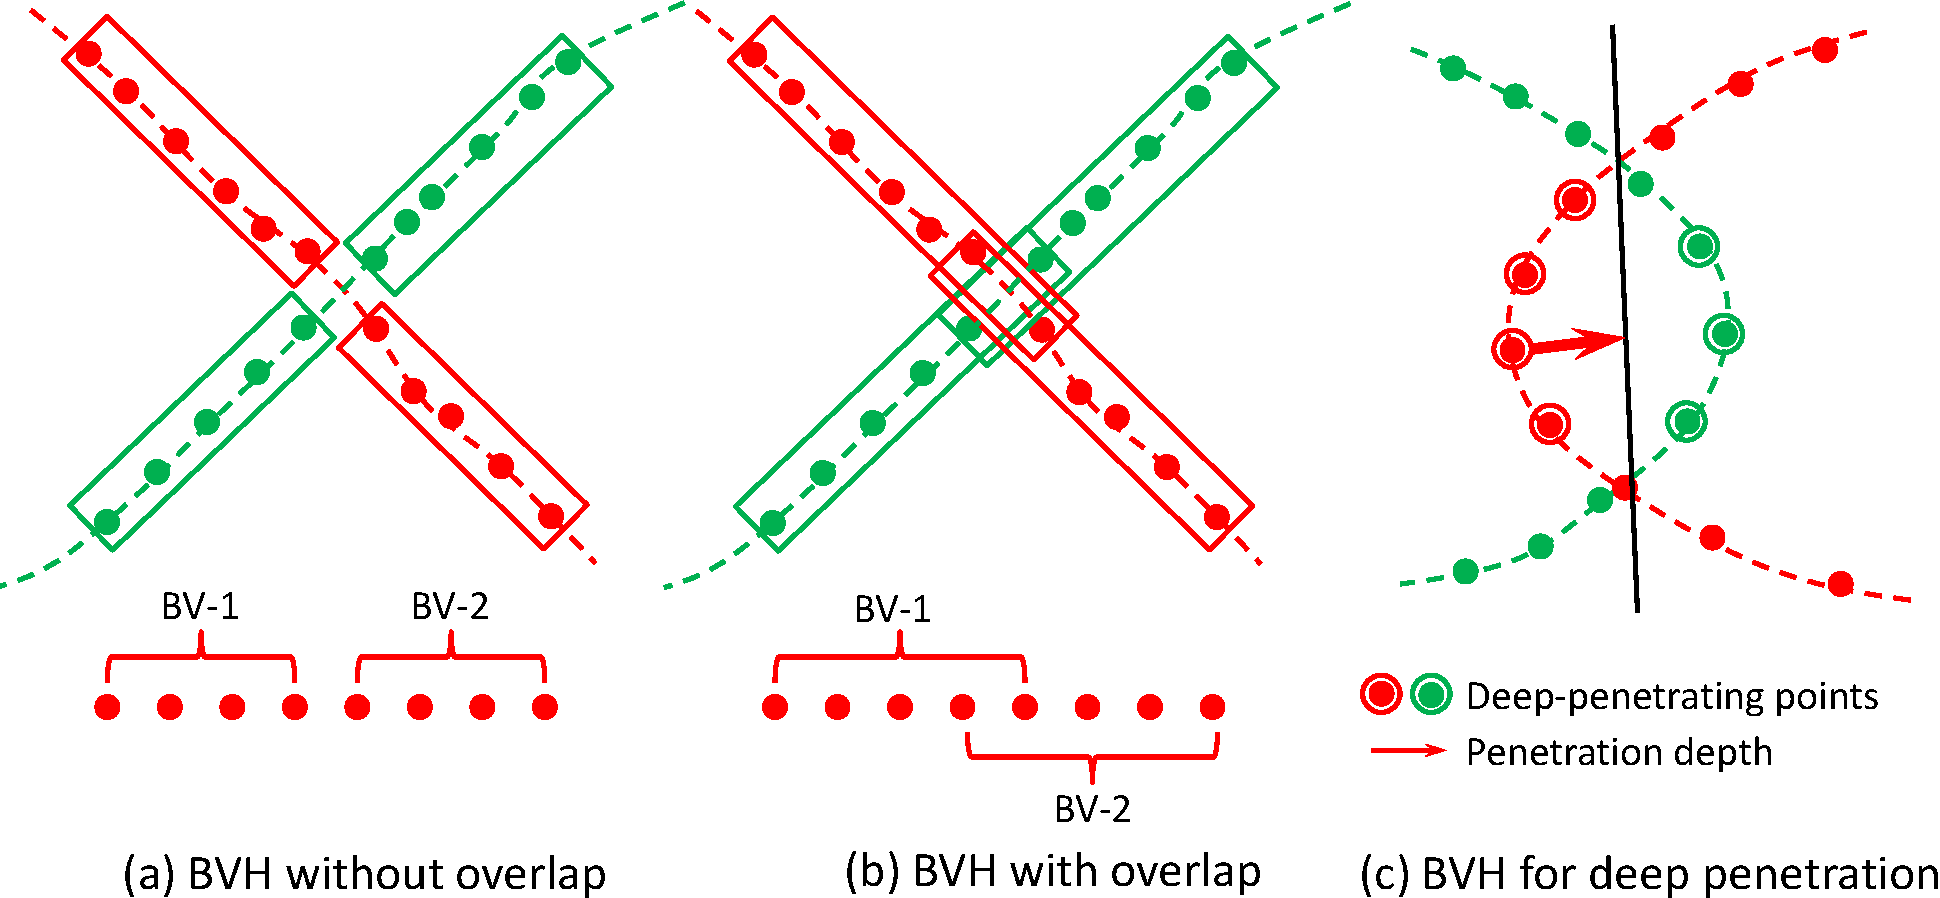
\includegraphics[width=0.9\linewidth]{figs/7/bvh_overlap.pdf}
  \caption[BVH acceleration for point-cloud collision]{\label{fig:7:bvh_overlap} Green and red points are the point clouds for two objects. Green and red intersecting lines are the underlying surfaces in collision. In (a), BVs split from the same parent node
  have no overlap and the collision detection algorithm returns collision-free. In (b), the BVs have overlap and the collision detection algorithm returns in-collision. (c) shows the deep-penetration case for which BVH may underestimate the collision probability for deeply-penetrating points.}
\end{figure}


\section{Implementation and Results}
\label{sec:7:results}
In this section, we describe some details of our implementation and evaluate its performance on several benchmarks.

\subsection{Implementation}
First, we discuss how to estimate the distribution of the underlying surface sample $p(\mathbf x_i')$. The mean of $p(\mathbf x_i')$ is $\mathbf x_i$, due to our unbiased assumption. We estimate the covariance $\Psi_i$ based on the formulation described in~\cite{Pauly:2004}:
\begin{equation}
\Psi_i = \frac{\sum_{j=1}^n (\mathbf x_j - \mathbf x_i)(\mathbf x_j - \mathbf x_i)^T \exp(-\|\mathbf x_i - \mathbf x_j\|^2 / \tau_i^2)}{\sum_{j=1}^n  \exp(-\|\mathbf x_i - \mathbf x_j\|^2 / \tau_i^2)},
\end{equation}
where $n$ is the total number of points and $\tau_i$ is a parameter used to downweight the influence of points that are too far away from $\mathbf x_i$. We set $\tau_i = \tau \cdot \eta_i$. $\tau$ is a global scale parameter, and the variable $\eta_i = \frac{r}{\sqrt{k}}$ denotes the local sample spacing estimated from a $k$-neighborhood, where $r$ is the radius of the enclosing sphere of the $k$-nearest neighbors of $\mathbf x_i$.

Our algorithm is based on machine learning techniques and includes some parameters that need to be tuned. Fortunately, we find that our method is not sensitive to the choice of parameters if we preprocess the data by scaling it to a $[0,1]^3$ volume in 3D. Scaling is considered important in terms of the robustness of SVM, especially for the non-linear case. Moreover, scaling also helps us in computing parameters that are suitable for point clouds with different sizes or configurations. In practice, scaling also changes the uncertainty of each point, so we need to update the noise level from $\widetilde{\Sigma}_i$ to $\mathbf S \widetilde{\Sigma}_i \mathbf S^T$, where $\mathbf S = \diag(s_1, s_2, s_3)$ is the scaling matrix.

We have used our algorithm on data captured using robot sensors. Note that our method is designed for noisy environments where the ground-truth for collision detection is unknown. In this case, exact collision algorithms are not applicable, since we do not have an exact representation of the environment.
Therefore, it is difficult to directly compare the quality or accuracy of our algorithm with prior methods. However, our method can guarantee: 1) For easy collision queries, i.e., when the distance between two collision-free objects is large or the two objects are in deep-penetration, our method will give collision probability near 0 or 1. In this case, only very large noise can reverse the outcome of the query. With this degree of large noise, our probabilistic algorithm would give the same (incorrect) result as the exact approach that first performs mesh reconstruction from the point clouds. 
2) For challenging queries, i.e., when two objects are almost in-contact or have a small penetration, our method computes a collision probability near 0.5, because these configurations are more susceptible to noise. Exact collision algorithms will still provide a yes-no result, but the accuracy of the exact algorithm is governed by the underlying sampling and mesh reconstruction algorithm. If a yes-no collision answer is required, our algorithm uses two thresholds $A \geq 0.5 \geq B$: if the collision probability is $>A$, we report \emph{collision-free}; if the collision probability is $< B$, we report \emph{in-collision}; if the collision probability is between $A$ and $B$, we report \emph{in-contact}. For example, when collision-avoidance is critical for underlying applications, we can use a large conservative value for $A$ and a small conservative value for $B$ to achieve better guarantees.

\subsection{Results}
We evaluate the performance of our algorithm on real-world point clouds as well as synthetic data sets. We also compare its accuracy with prior collision
detection techniques. The running time of our probabilistic algorithm is similar to that of exact collision detection algorithms and varies based on the
number of primitives and their relative configurations.

\begin{figure}[!htb]
\centering
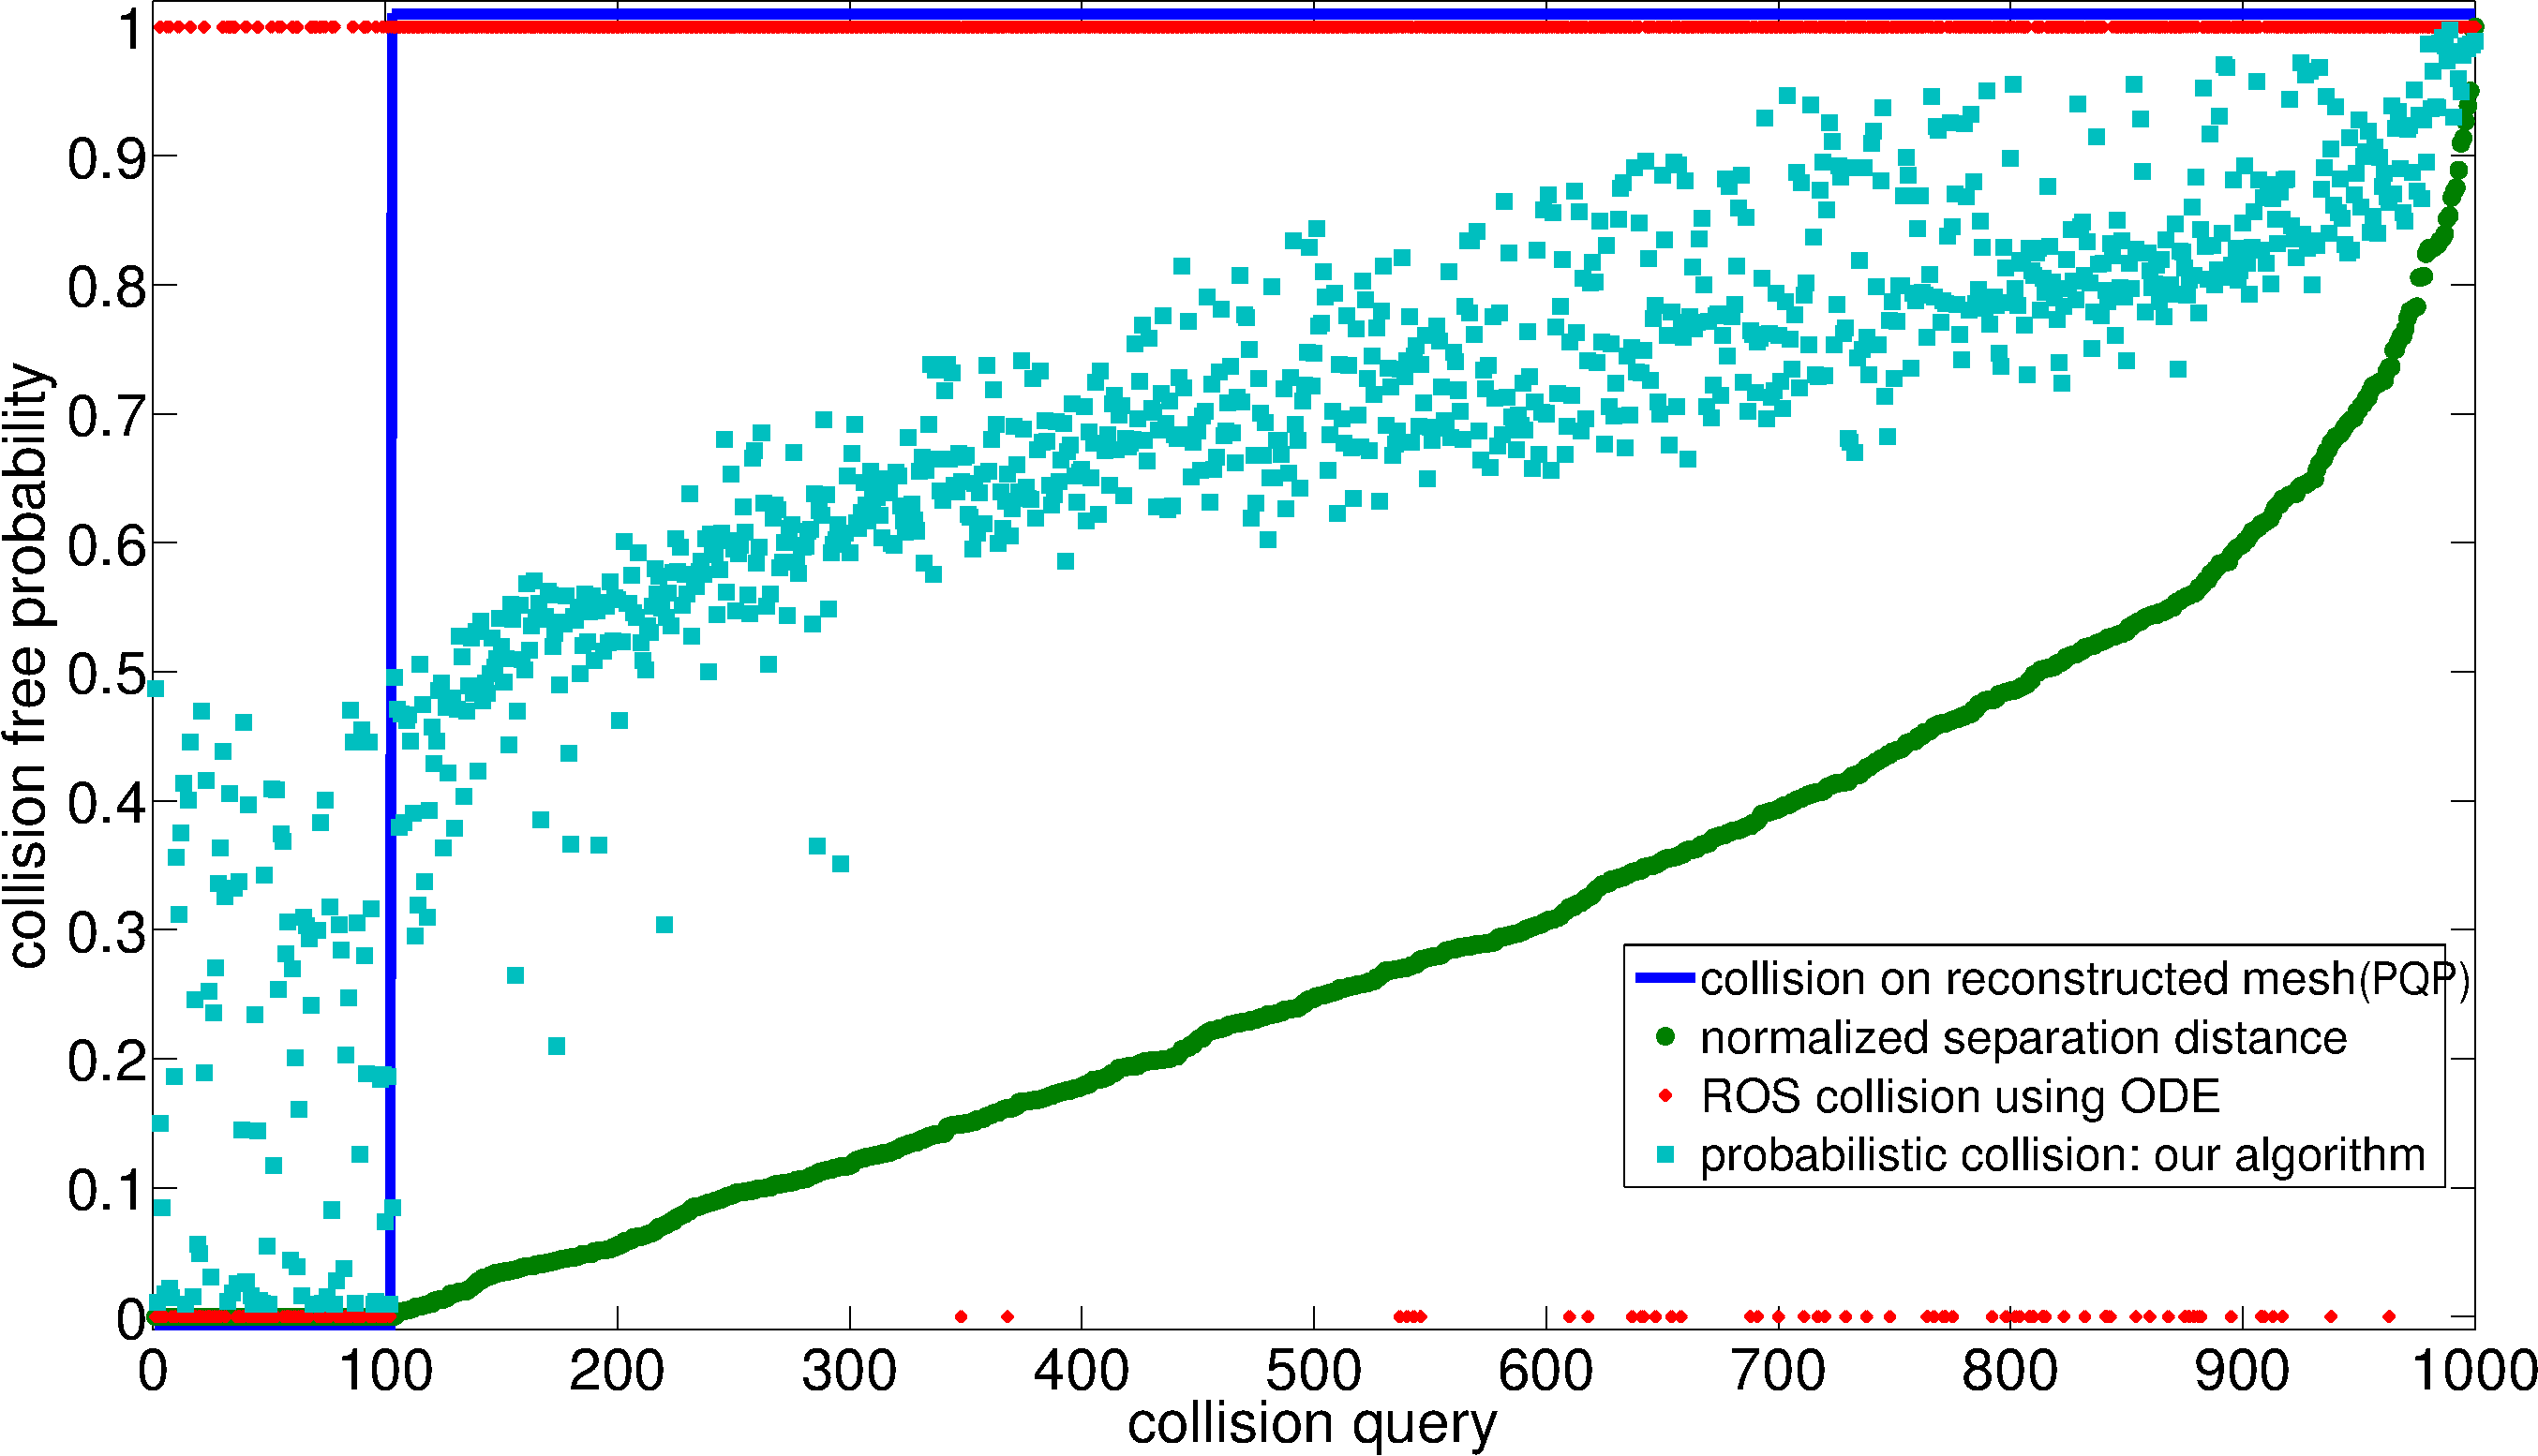
\includegraphics[width=0.79\linewidth]{figs/7/pr2res.pdf}
\caption[Comparison of collision checking algorithms with and without considering data uncertainty on point-cloud data generated by PR2 robot sensor]{\label{fig:7:res2} Comparison on point-cloud data generated by the PR2 robot's sensor: we use our probabilistic collision detection on the noisy point
cloud vs. results computed by the ODE package used in ROS vs. exact collision and distance queries on the reconstructed mesh model. Our results on the point cloud
are more robust than that of the ODE package.}
\end{figure}


\begin{figure}[!htb]
  \centering
  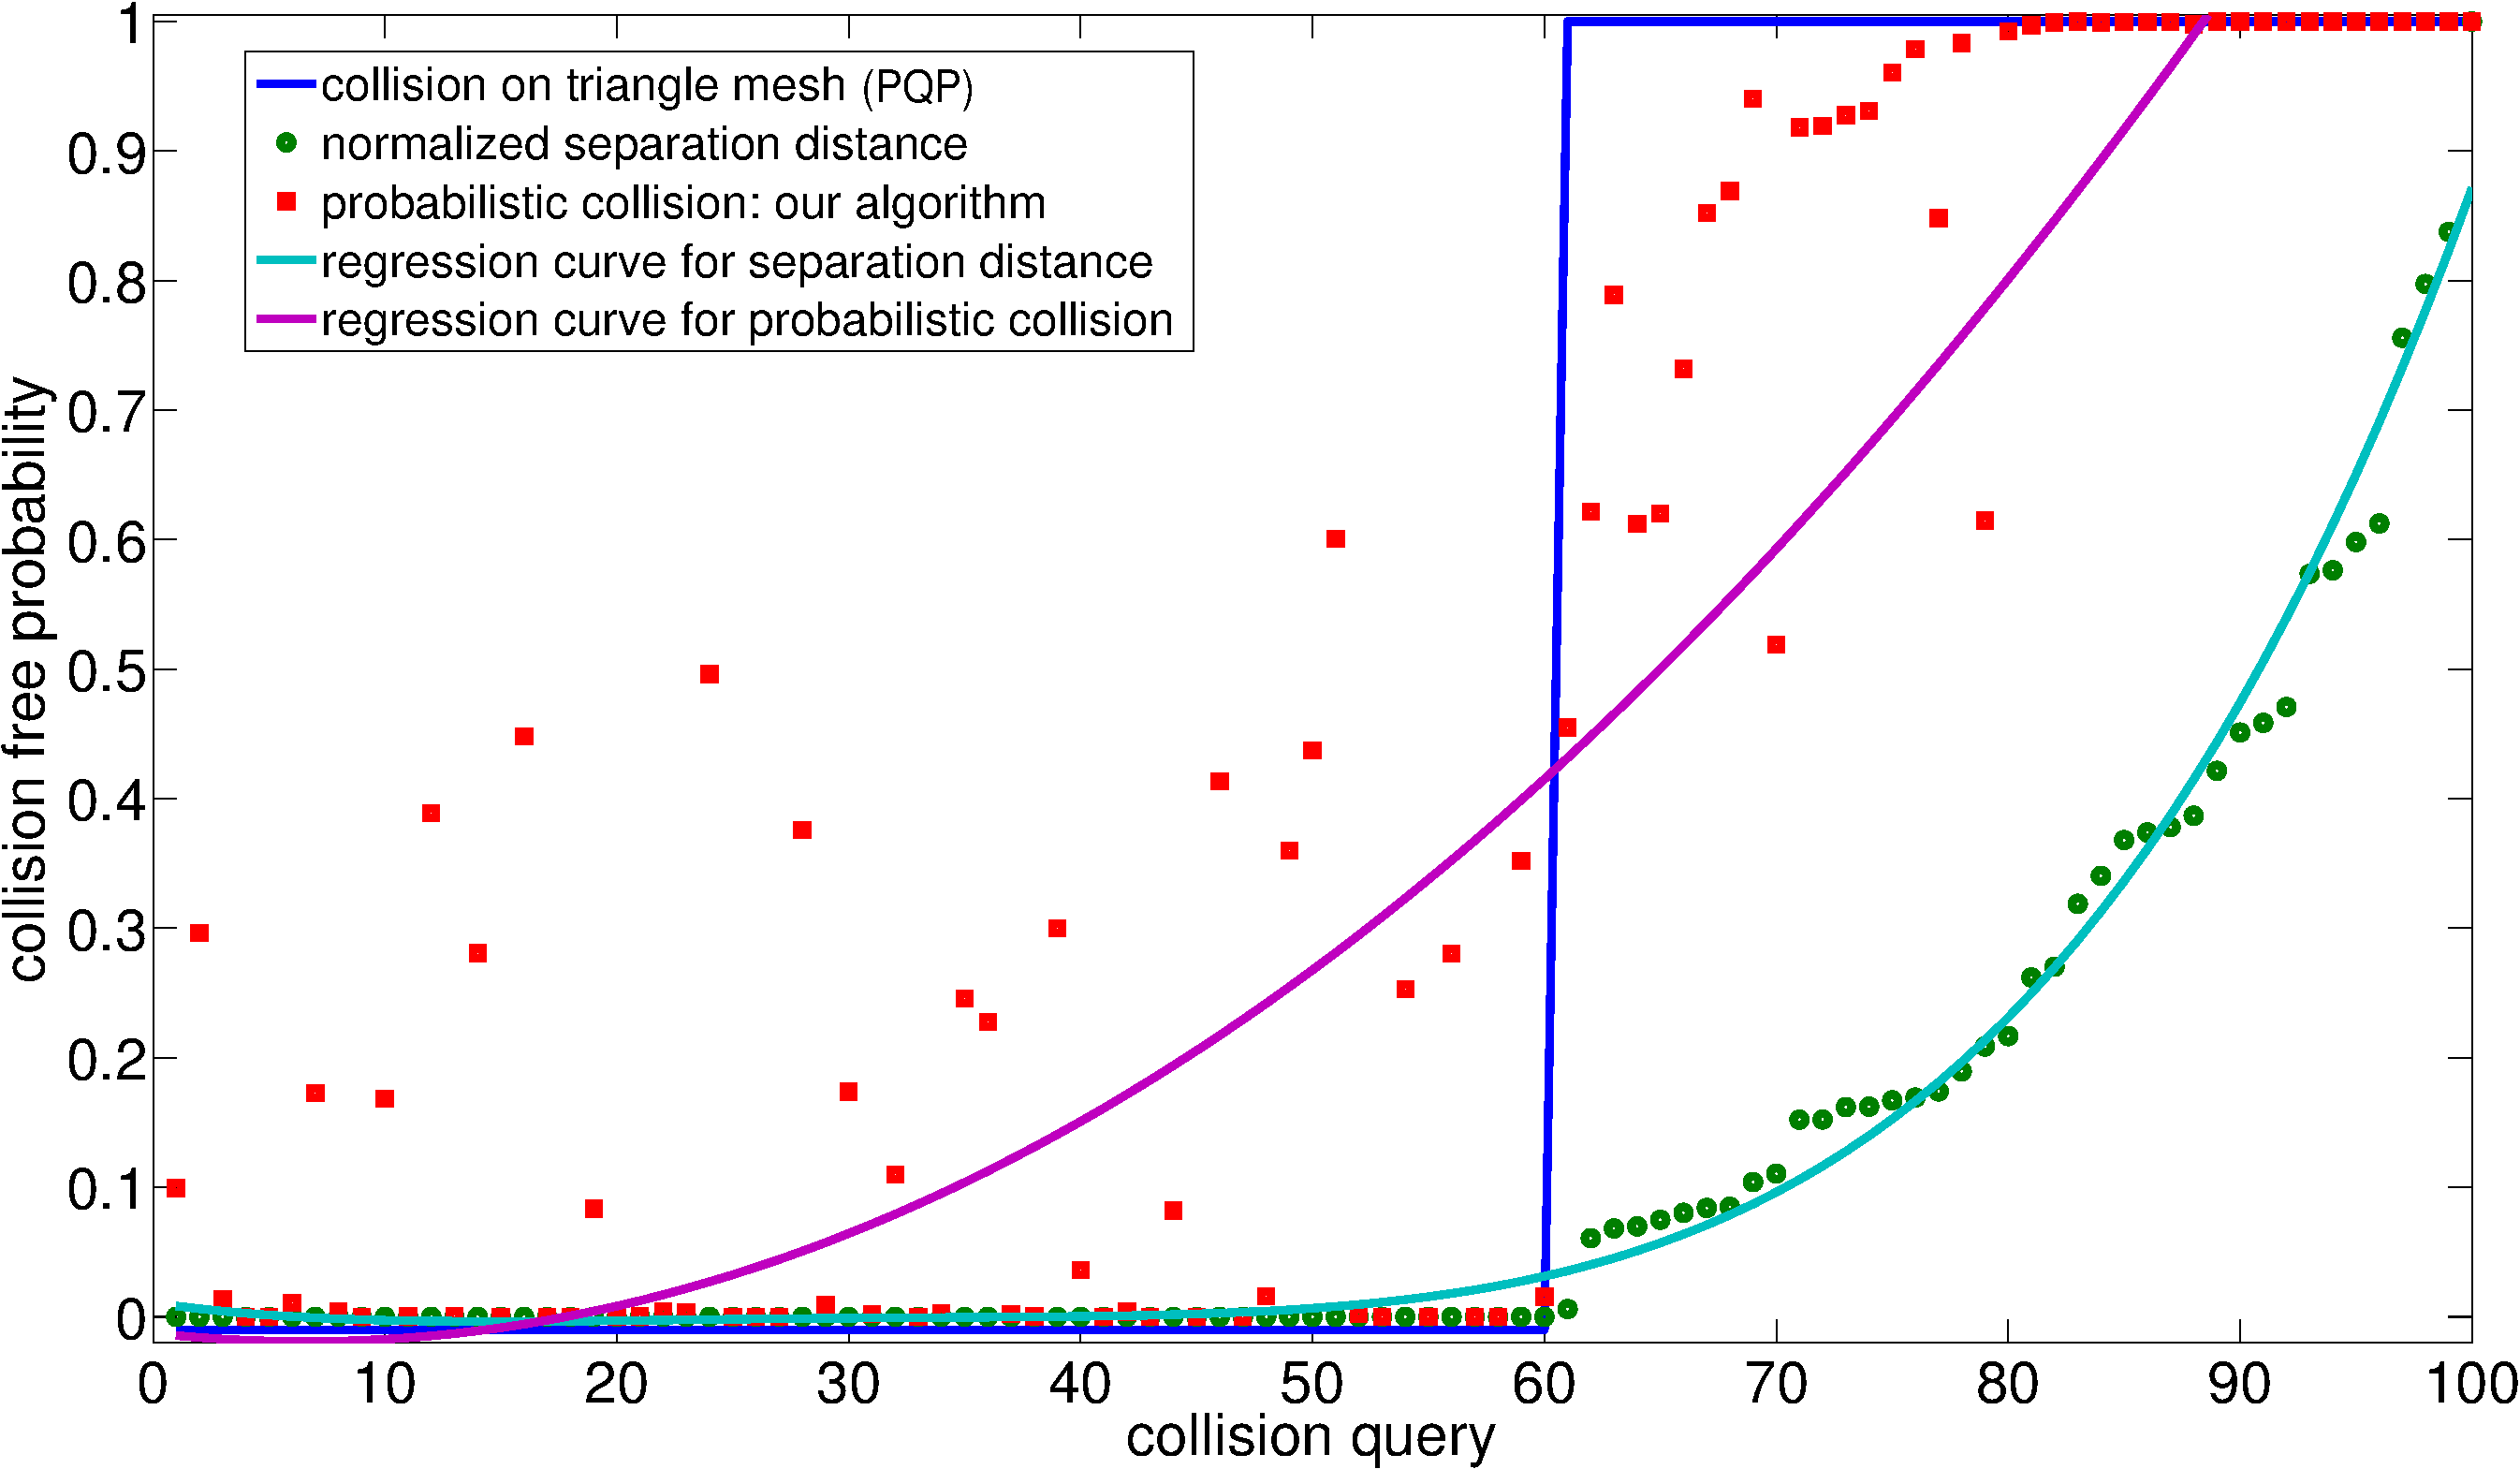
\includegraphics[width=0.79\linewidth]{figs/7/smallnoise.pdf}
  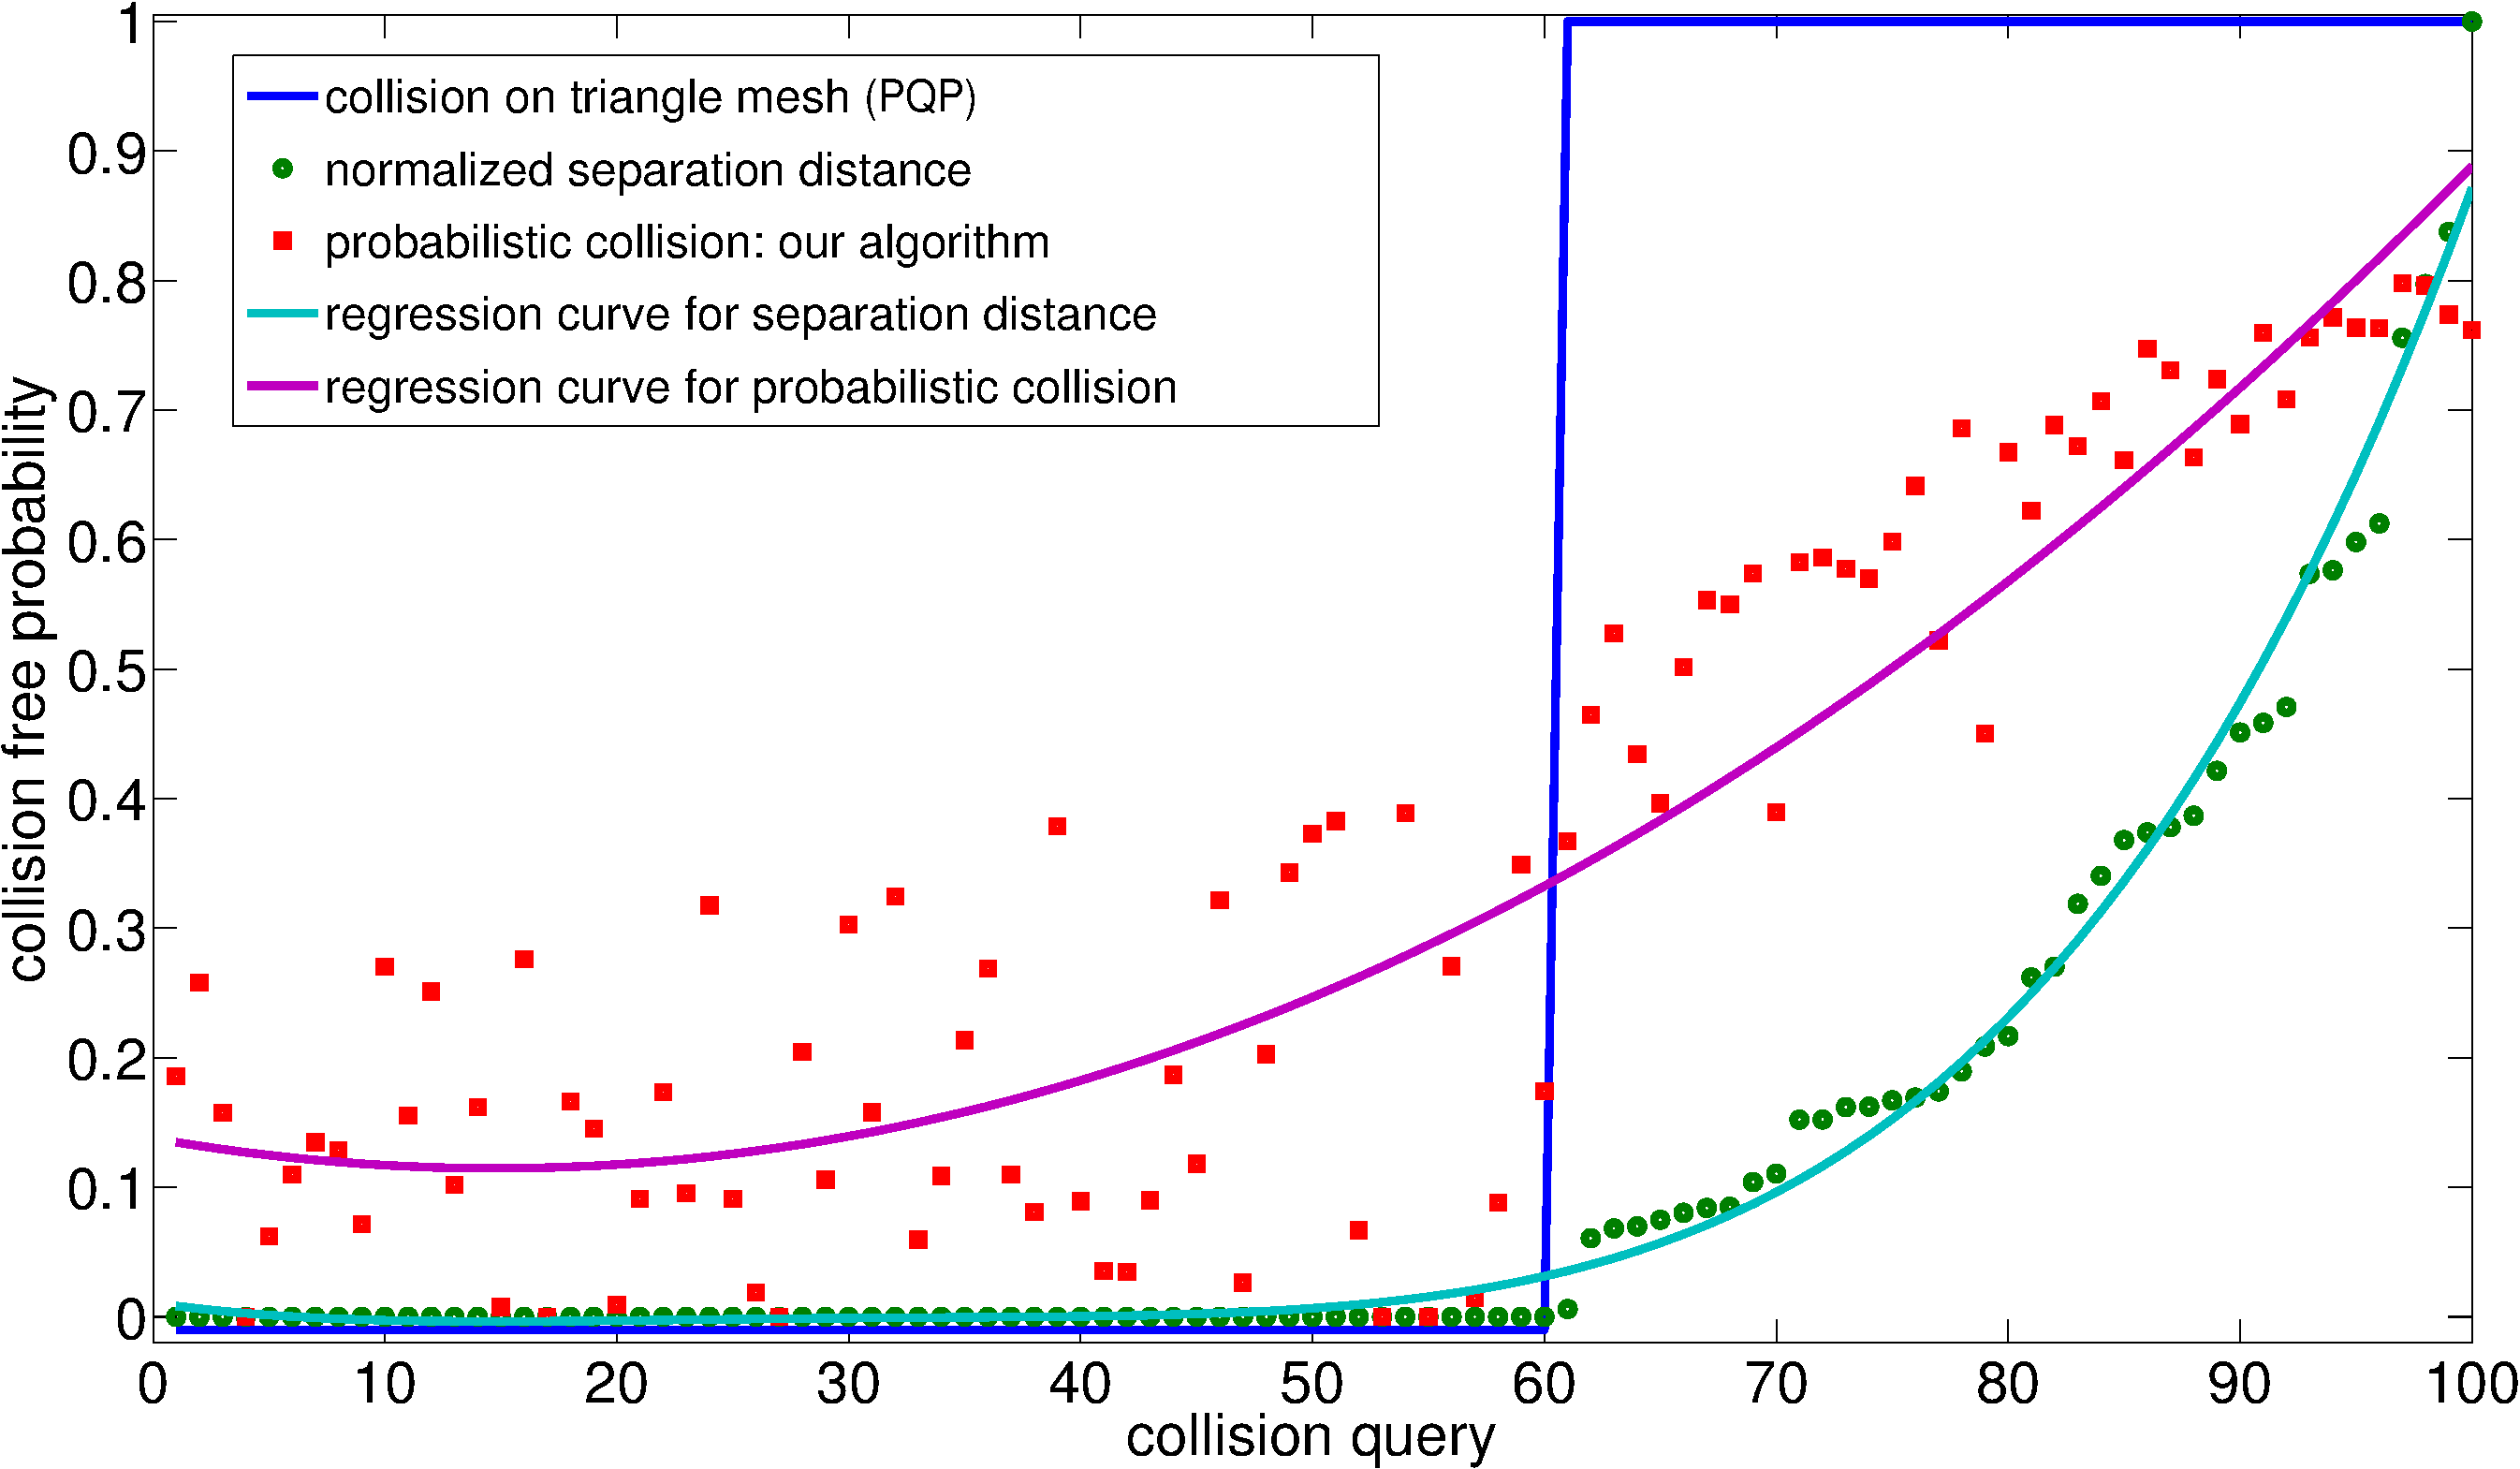
\includegraphics[width=0.79\linewidth]{figs/7/largenoise.pdf}
  \caption[Comparison between the results for $100$ random queries between prior collision detection algorithms for exact triangle meshes and our
  algorithm on the point clouds]{\label{fig:7:res1} Comparison between the results for $100$ random queries between prior collision detection algorithms for exact triangle meshes and our
  algorithm on the point clouds (generated by sampling and adding noise). We show the results of exact collision detection and separation distance as well. If the noise in
  the point cloud is small (the upper figure), our method returns a $0$ or $1$ collision probability for most queries. When the queries correspond to a small separation distance or penetration depth (i.e., difficult cases), our algorithm computes a collision-free probability close to $0.5$.
  Furthermore, the collision-free probability is higher when the separation distance is large for non-overlapping objects. If
  the noise is large (the bottom figure), fewer queries return a $0$ or $1$ collision probability. We see a close correlation between the regression
  curves computed by our algorithm and the exact queries on these synthetic datasets.}
\end{figure}

\begin{figure}[!htb]
  \centering
  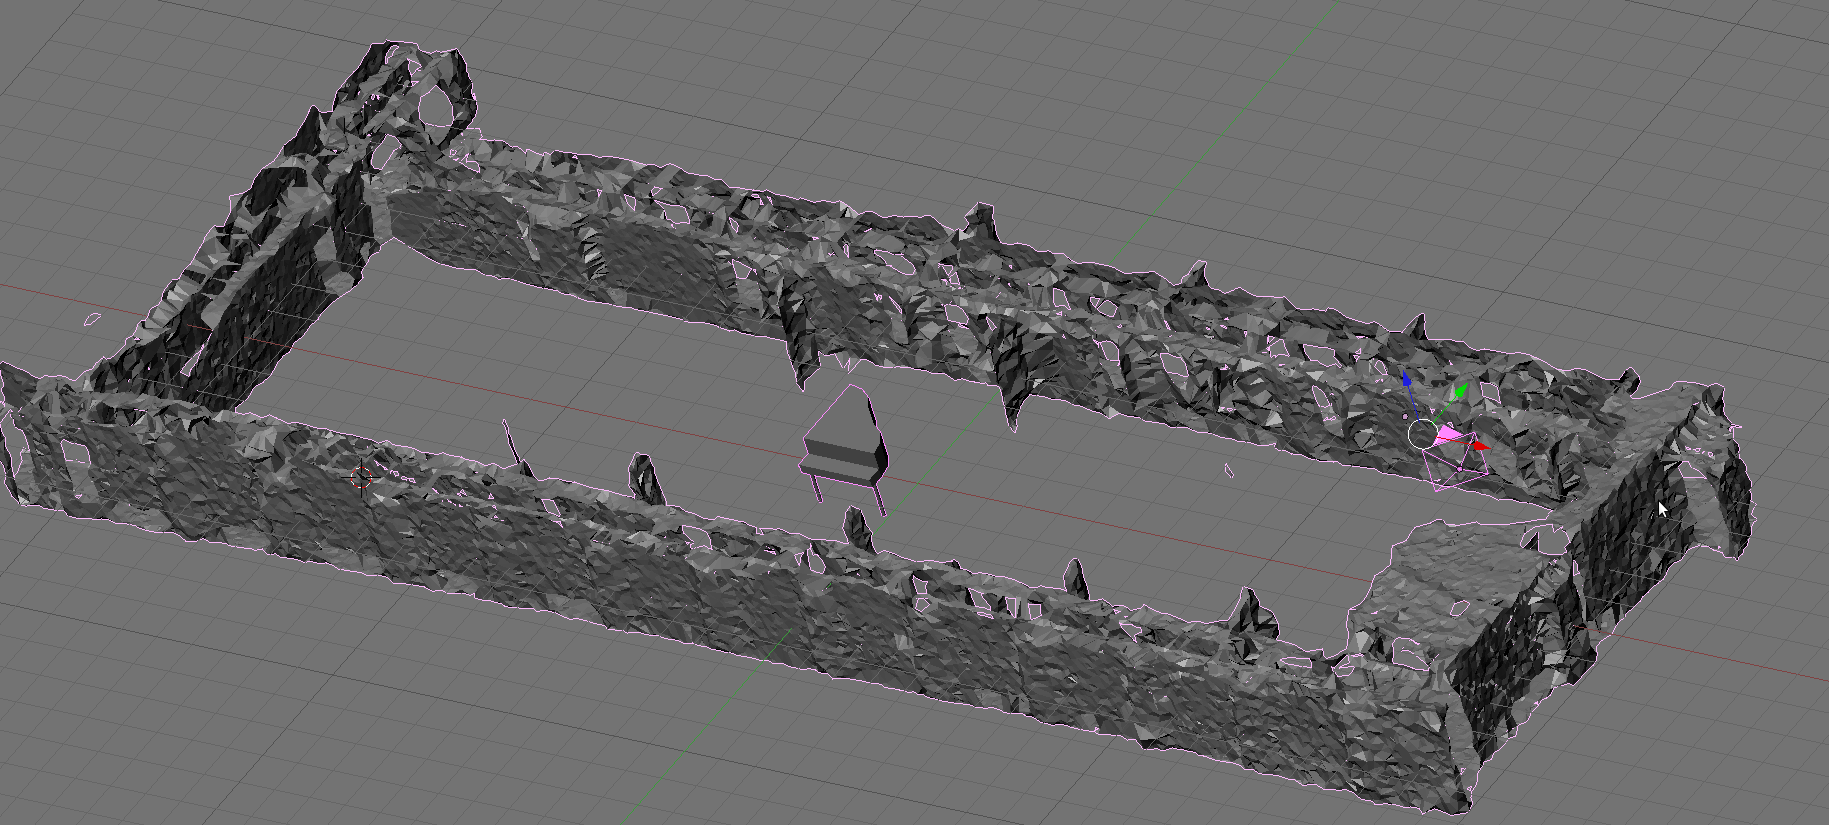
\includegraphics[width=0.79\linewidth]{figs/7/kinect.png}
  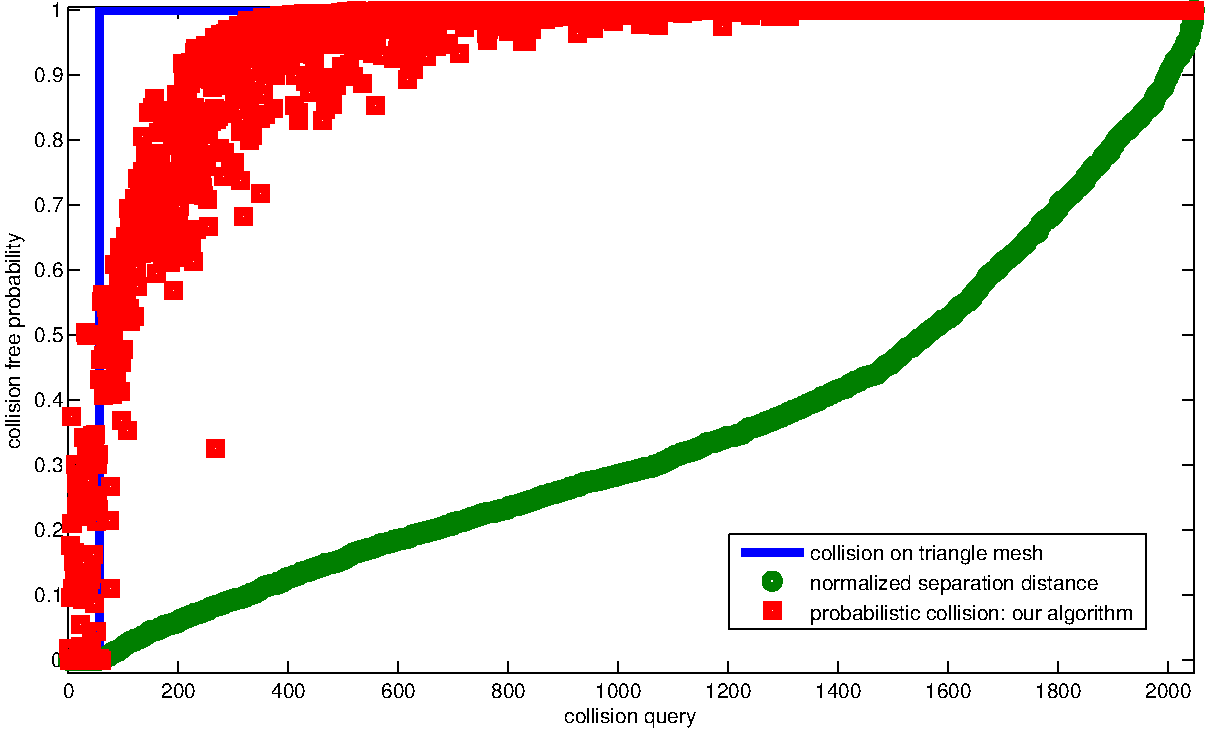
\includegraphics[width=0.79\linewidth]{figs/7/kinect.pdf}
  \caption[Comparison between the results for $100$ random queries between prior collision detection algorithms for exact triangle meshes and our
  algorithm on the Kinect data]{\label{fig:7:res3} (a) Kinect data; (b) Robust Classification of contact status between the point clouds generated using Kinect.}
\end{figure}



We evaluated the performance of our algorithm on a synthetic data set corresponding to a moving piano in a room with tables.
We generated a point cloud by sampling the polygons and adding some noise. We used the PQP package to perform exact collision detection and separation
distance query between the exact, triangulated model and compared the results with probabilistic collision detection on the resulting point cloud (Figure~\ref{fig:7:res1}). We see a high correlation between our results and the actual separation distance, and it varies based on the level of noise.
This shows that our approach is quite robust and even works well in degenerate configurations, e.g., when the two objects are barely touching or very close to each other. Such configurations are more susceptible to noise and the exact collision detection algorithms are very sensitive to these configurations.


We have applied our probabilistic collision detection to the point cloud data generated for manipulation using the PR2 robot. Point cloud data on the PR2 robot is generated from a scanning laser range finder (\emph{Hokuyo Top-URG(UTM-30LX)}) and a stereo camera (\emph{WGE-100}), which is combined with an active texture projector to obtain good 3D data from untextured objects. The robot is placed in front of a table with multiple household objects (e.g., bowls, cans) on the table at a distance of about 1.5 m from the robot's sensors. The point clouds are a discretized (about +/-1.5 cm in range) representation of the real environment and are generated periodically by each sensor. The data is noisy and exhibits speckles, especially in the vicinity of boundaries of objects and boundaries of the sensor's field of view. The sensors are calibrated with respect to each other and the arms using a known calibration pattern. The known position of the arms, measured using encoders, is used to filter out the points corresponding to the arms from the point clouds obtained by the sensors. Typical point clouds generated by the stereo sensors on the PR2 robot have more than $40,000$ points and are generated at 20 Hz. Point clouds generated by the laser range scanners typically have about $10,000$ points. Data from the point clouds is aggregated into a {\em collision map} representation. The collision map is a 3-dimensional occupancy grid maintained at a fixed resolution. The resulting collision maps are at 1 cm resolution and have about $2,000$ occupied cells. A complete triangulated mesh representation of the robot, including the arms and the gripper, is also available as input for the collision checker.

There are very few algorithms or systems available for collision checking between noisy point clouds. As a result, we resort to comparing our algorithm with the implementation in ROS (based on ODE) and exact collision detection on reconstructed meshes.

The collision checking procedures used in ROS are currently based on the collision checking implementation in the ODE software package. The input to the collision checker includes mesh models for the robot and objects in the environment, as well as the collision map. The points in the collision map are represented as axis-aligned box primitives whose length is equal to the resolution at which the collision map is maintained. The current representation of the collision space considers every point in the collision map to be a potential obstacle. Thus, noise in the sensor data can frequently lead to false positives, i.e., the detection of potential collisions in parts of the environment where there are no obstacles. There is no robust criterion to compute the box size (e.g., a function of noise), so we cannot compare all the features of our method with ODE collision checking. We also use a reconstruction algorithm to compute a triangle mesh from the point clouds and perform triangle-based collision as well as separation distance computation using PQP. This formulation only provides an approximation of the ground truth and is used to evaluate the robustness of our algorithm.

As shown in Figure~\ref{fig:7:res2}, our result is comparable to in quality with the exact collision detection algorithm, especially for computing the separation distance. Furthermore, we notice that the collision probability of our approach changes slowly when the noise increases. It is more robust than the yes-no result computed by ODE on the point clouds, which is likely to frequently switch between collision-free and in-contact configurations when the noise level changes.
Moreover, from Figures~\ref{fig:7:res2} and~\ref{fig:7:res1}, we observe that configurations with the same distances to the obstacles can have large spread in the computed collision probabilities. The reason is that distance is only a partial measurement of collision status, while our collision probability is a more complete description about collision status and provides more detailed information about the relative configurations.

For one query, our method needs about 500-1000 ms for about 10,000 points on one Intel Core i7 3.2GHz CPU, based on BVH acceleration. It is about 5-10 times slower than optimized collision packages on models with 10K triangles (e.g., PQP can compute collisions in such situations in about 50ms-100ms). However, the reconstruction algorithms take more than 10 seconds to compute the triangulated mesh from the point cloud. Moreover, our current implementation can be optimized in several ways, such as replacing the non-linear kernel by the approximated linear kernel~\cite{Ali:nips:2007} and using more efficient SVM methods designed for large scale data~\cite{Fan:2008:LLL}. We expect an optimized probabilistic collision method to have similar speed to the PQP algorithm. Furthermore, our approach can provide more detailed information and can be easily combined with planning and reasoning algorithms. For example, we can combine it with trajectory optimization algorithms (e.g., CHOMP~\cite{Ratliff:2009}, STOMP~\cite{Mrinal:2011}) to find a smooth path that has a minimum probability of colliding with the obstacles.

Additionally, we show in Figure~\ref{fig:7:res3}(b) the collision results between the PR2 robot and the Kinect data shown in Figure~\ref{fig:7:res3}(a). We compare the result of our method with exact collision detection on reconstructed meshes.





\section{Conclusions and Future Work}

We have presented a novel and robust method for contact computation using noisy point cloud data, by applying machine learning methods.
We reformulate collision detection as a two-classification problem and compute the collision probability at each point using
support vector machines. This algorithm can be accelerated by using bounding volume hierarchies and performing a stochastic traversal. We have tested
the results on synthetic and real-world data sets, and the preliminary results are promising.

There are many avenues for future work. We need to test the performance on different robotic systems and evaluate its performance
on tasks such as planning and grasping.
It would be useful to extend this approach to continuous collision checking, which takes into account the motion of the robot
between discrete intervals along its path. Similar probabilistic methods can also be developed for other queries,
including separation and penetration depth computation. Finally, we are interested in improving the algorithm to handle dynamic environments where points may change position or can be added or removed from the environment due to movement, occlusion, or incremental data, based on incremental SVM~\cite{Gert:nips:2001} and BVH refitting techniques~\cite{Lauterbach10}.

